% Options for packages loaded elsewhere
\PassOptionsToPackage{unicode}{hyperref}
\PassOptionsToPackage{hyphens}{url}
%
\documentclass[
]{book}
\usepackage{amsmath,amssymb}
\usepackage{iftex}
\ifPDFTeX
  \usepackage[T1]{fontenc}
  \usepackage[utf8]{inputenc}
  \usepackage{textcomp} % provide euro and other symbols
\else % if luatex or xetex
  \usepackage{unicode-math} % this also loads fontspec
  \defaultfontfeatures{Scale=MatchLowercase}
  \defaultfontfeatures[\rmfamily]{Ligatures=TeX,Scale=1}
\fi
\usepackage{lmodern}
\ifPDFTeX\else
  % xetex/luatex font selection
\fi
% Use upquote if available, for straight quotes in verbatim environments
\IfFileExists{upquote.sty}{\usepackage{upquote}}{}
\IfFileExists{microtype.sty}{% use microtype if available
  \usepackage[]{microtype}
  \UseMicrotypeSet[protrusion]{basicmath} % disable protrusion for tt fonts
}{}
\makeatletter
\@ifundefined{KOMAClassName}{% if non-KOMA class
  \IfFileExists{parskip.sty}{%
    \usepackage{parskip}
  }{% else
    \setlength{\parindent}{0pt}
    \setlength{\parskip}{6pt plus 2pt minus 1pt}}
}{% if KOMA class
  \KOMAoptions{parskip=half}}
\makeatother
\usepackage{xcolor}
\usepackage{color}
\usepackage{fancyvrb}
\newcommand{\VerbBar}{|}
\newcommand{\VERB}{\Verb[commandchars=\\\{\}]}
\DefineVerbatimEnvironment{Highlighting}{Verbatim}{commandchars=\\\{\}}
% Add ',fontsize=\small' for more characters per line
\usepackage{framed}
\definecolor{shadecolor}{RGB}{248,248,248}
\newenvironment{Shaded}{\begin{snugshade}}{\end{snugshade}}
\newcommand{\AlertTok}[1]{\textcolor[rgb]{0.94,0.16,0.16}{#1}}
\newcommand{\AnnotationTok}[1]{\textcolor[rgb]{0.56,0.35,0.01}{\textbf{\textit{#1}}}}
\newcommand{\AttributeTok}[1]{\textcolor[rgb]{0.13,0.29,0.53}{#1}}
\newcommand{\BaseNTok}[1]{\textcolor[rgb]{0.00,0.00,0.81}{#1}}
\newcommand{\BuiltInTok}[1]{#1}
\newcommand{\CharTok}[1]{\textcolor[rgb]{0.31,0.60,0.02}{#1}}
\newcommand{\CommentTok}[1]{\textcolor[rgb]{0.56,0.35,0.01}{\textit{#1}}}
\newcommand{\CommentVarTok}[1]{\textcolor[rgb]{0.56,0.35,0.01}{\textbf{\textit{#1}}}}
\newcommand{\ConstantTok}[1]{\textcolor[rgb]{0.56,0.35,0.01}{#1}}
\newcommand{\ControlFlowTok}[1]{\textcolor[rgb]{0.13,0.29,0.53}{\textbf{#1}}}
\newcommand{\DataTypeTok}[1]{\textcolor[rgb]{0.13,0.29,0.53}{#1}}
\newcommand{\DecValTok}[1]{\textcolor[rgb]{0.00,0.00,0.81}{#1}}
\newcommand{\DocumentationTok}[1]{\textcolor[rgb]{0.56,0.35,0.01}{\textbf{\textit{#1}}}}
\newcommand{\ErrorTok}[1]{\textcolor[rgb]{0.64,0.00,0.00}{\textbf{#1}}}
\newcommand{\ExtensionTok}[1]{#1}
\newcommand{\FloatTok}[1]{\textcolor[rgb]{0.00,0.00,0.81}{#1}}
\newcommand{\FunctionTok}[1]{\textcolor[rgb]{0.13,0.29,0.53}{\textbf{#1}}}
\newcommand{\ImportTok}[1]{#1}
\newcommand{\InformationTok}[1]{\textcolor[rgb]{0.56,0.35,0.01}{\textbf{\textit{#1}}}}
\newcommand{\KeywordTok}[1]{\textcolor[rgb]{0.13,0.29,0.53}{\textbf{#1}}}
\newcommand{\NormalTok}[1]{#1}
\newcommand{\OperatorTok}[1]{\textcolor[rgb]{0.81,0.36,0.00}{\textbf{#1}}}
\newcommand{\OtherTok}[1]{\textcolor[rgb]{0.56,0.35,0.01}{#1}}
\newcommand{\PreprocessorTok}[1]{\textcolor[rgb]{0.56,0.35,0.01}{\textit{#1}}}
\newcommand{\RegionMarkerTok}[1]{#1}
\newcommand{\SpecialCharTok}[1]{\textcolor[rgb]{0.81,0.36,0.00}{\textbf{#1}}}
\newcommand{\SpecialStringTok}[1]{\textcolor[rgb]{0.31,0.60,0.02}{#1}}
\newcommand{\StringTok}[1]{\textcolor[rgb]{0.31,0.60,0.02}{#1}}
\newcommand{\VariableTok}[1]{\textcolor[rgb]{0.00,0.00,0.00}{#1}}
\newcommand{\VerbatimStringTok}[1]{\textcolor[rgb]{0.31,0.60,0.02}{#1}}
\newcommand{\WarningTok}[1]{\textcolor[rgb]{0.56,0.35,0.01}{\textbf{\textit{#1}}}}
\usepackage{longtable,booktabs,array}
\usepackage{calc} % for calculating minipage widths
% Correct order of tables after \paragraph or \subparagraph
\usepackage{etoolbox}
\makeatletter
\patchcmd\longtable{\par}{\if@noskipsec\mbox{}\fi\par}{}{}
\makeatother
% Allow footnotes in longtable head/foot
\IfFileExists{footnotehyper.sty}{\usepackage{footnotehyper}}{\usepackage{footnote}}
\makesavenoteenv{longtable}
\usepackage{graphicx}
\makeatletter
\def\maxwidth{\ifdim\Gin@nat@width>\linewidth\linewidth\else\Gin@nat@width\fi}
\def\maxheight{\ifdim\Gin@nat@height>\textheight\textheight\else\Gin@nat@height\fi}
\makeatother
% Scale images if necessary, so that they will not overflow the page
% margins by default, and it is still possible to overwrite the defaults
% using explicit options in \includegraphics[width, height, ...]{}
\setkeys{Gin}{width=\maxwidth,height=\maxheight,keepaspectratio}
% Set default figure placement to htbp
\makeatletter
\def\fps@figure{htbp}
\makeatother
\setlength{\emergencystretch}{3em} % prevent overfull lines
\providecommand{\tightlist}{%
  \setlength{\itemsep}{0pt}\setlength{\parskip}{0pt}}
\setcounter{secnumdepth}{5}
\newlength{\cslhangindent}
\setlength{\cslhangindent}{1.5em}
\newlength{\csllabelwidth}
\setlength{\csllabelwidth}{3em}
\newlength{\cslentryspacingunit} % times entry-spacing
\setlength{\cslentryspacingunit}{\parskip}
\newenvironment{CSLReferences}[2] % #1 hanging-ident, #2 entry spacing
 {% don't indent paragraphs
  \setlength{\parindent}{0pt}
  % turn on hanging indent if param 1 is 1
  \ifodd #1
  \let\oldpar\par
  \def\par{\hangindent=\cslhangindent\oldpar}
  \fi
  % set entry spacing
  \setlength{\parskip}{#2\cslentryspacingunit}
 }%
 {}
\usepackage{calc}
\newcommand{\CSLBlock}[1]{#1\hfill\break}
\newcommand{\CSLLeftMargin}[1]{\parbox[t]{\csllabelwidth}{#1}}
\newcommand{\CSLRightInline}[1]{\parbox[t]{\linewidth - \csllabelwidth}{#1}\break}
\newcommand{\CSLIndent}[1]{\hspace{\cslhangindent}#1}
\usepackage{mathrsfs}
\usepackage{caption}
\ifLuaTeX
  \usepackage{selnolig}  % disable illegal ligatures
\fi
\IfFileExists{bookmark.sty}{\usepackage{bookmark}}{\usepackage{hyperref}}
\IfFileExists{xurl.sty}{\usepackage{xurl}}{} % add URL line breaks if available
\urlstyle{same}
\hypersetup{
  pdftitle={Applied Malaria Dynamics},
  pdfauthor={David L. Smith and the RAMP Team},
  hidelinks,
  pdfcreator={LaTeX via pandoc}}

\title{Applied Malaria Dynamics}
\usepackage{etoolbox}
\makeatletter
\providecommand{\subtitle}[1]{% add subtitle to \maketitle
  \apptocmd{\@title}{\par {\large #1 \par}}{}{}
}
\makeatother
\subtitle{Dynamical Systems for Adaptive Malaria Control}
\author{David L. Smith and the RAMP Team}
\date{2023-06-21}

\begin{document}
\maketitle

{
\setcounter{tocdepth}{2}
\tableofcontents
}
\hypertarget{foreword}{%
\chapter*{Foreword}\label{foreword}}
\addcontentsline{toc}{chapter}{Foreword}

A large fraction of my time over the past 20 years has been devoted to learning about mathematical models of malaria epidemiology, transmission dynamics, mosquito ecology, vector control, and the evolution of resistance. All the time I was building and analyzing models, I was looking for a way of organizing and applying the rich body of theory developed over more than a century of malaria research, starting with Ross and Macdonald {[}\protect\hyperlink{ref-SmithDL2012_RossMacdonald}{1}{]}.
A new framework would integrate the concepts and models that have influenced malaria through the present day {[}\protect\hyperlink{ref-SmithNR2018AgentbasedModels}{2},\protect\hyperlink{ref-ReinerRCJ2013SystematicReview}{\textbf{ReinerRCJ2013SystematicReview?}}{]}, and it might even serve as a platform for recasting a theory of malaria epidemiology, transmission dynamics, and control {[}\protect\hyperlink{ref-SmithDL2014_Recasting}{3}{]}.

The goal was to build a framework that could serve malaria policy. Policy discussions might need the math, but the discussion should never be about the math. There were some core challenges, but if we could solve those, we could make the math easier to use so that discussions would focus on the issues that mattered. Ideally, the framework could be taken up and used by teams of local experts working in their own countries to reduce the burden of malaria and plan for its elimination.

I wanted the new framework to be \emph{extensible,} with \emph{plug-and-play} modularity (for major dynamical components), and with structural flexibility. It should have the capability of scaling down for fine-grained spatial simulations {[}\protect\hyperlink{ref-CarterR2002SpatialSimulation}{4}--\protect\hyperlink{ref-PerkinsTA2013HeterogeneityMixing}{6}{]}, or scaling up to understand or analyze regional processes and the emerging patterns {[}\protect\hyperlink{ref-TatemAJ2010InternationalPopulation}{7}{]}. To serve the needs of malaria programs, a framework would need built-in support for exogenous forcing by weather and vector control to model malaria as a changing baseline modified by control. To get integrated vector control right, we went all in on mosquito ecology with an individual-based simulation model with exquisite biological detail {[}\protect\hyperlink{ref-WuSL2020MBITES}{8}{]}, which inspired new ideas about mosquito search and a new base model for mosquito ecology and behavior. To serve programmatic needs, we needed algorithms that could address the durability of a unit of vector control -- coverage could decay over time through loss (\emph{e.g.} bed nets) or waning potency. To make all the pieces fit together, we needed interfaces that could connect up models in a generic way; in the design phase, we worked with two model families for each major dynamical component -- one that was dead simple, and one that had a was highly realistic. In some cases, the interface designs called for development of new algorithms: blood feeding, egg laying, environmental heterogeneity, human mobility, and mosquito dispersal. In making a master list to test the framework's extensibility, we found that some odd cases that needed to pass information among components -- endectocides and auto-disseminated larvicides -- but it was easy enough to accommodate these. These models needed supporting theory. We wanted the software to help understand thresholds, so we wrote the routines that would compute thresholds for malaria transmission in heterogeneous systems, when appropriate.

Sometime in the fall of 2022, the last few pieces came together. We published the first versions of \href{https://cran.r-project.org/package=MicroMoB}{MicroMoB} and \href{https://CRAN.R-project.org/package=exDE}{exDE} at CRAN. We submitted a paper to PLoS Computational Biology {[}\protect\hyperlink{ref-WuSL2022SpatialDynamics}{9}{]}. Then it was time to write this book.

With the software developed, we have the capability of building models that are up to the task of guiding malaria policy. The advantage of using the framework and accompanying software is that we found design solutions after discovering (usually the hard way) the potential pitfalls that arise when combining models. The framework took longer to developed than I had expected, in part, because there were more pitfalls than we had anticipated.

This book shows, through examples, how to use the software to build malaria models. Even without the software, it fills a gap for students who have taken an introduction to mathematical epidemiology or infectious disease modeling and want to go on in malaria. What are all the special topics that would need to be covered to build models that could be needed in malaria? This book \emph{could} be the basis for such a course, if there were ever enough students. Since there will probably never be enough graduate students at my university who are interested in applied malaria dynamics, the material is being developed for any student anywhere. This book teaches how to build models for malaria policy, but it stops short of applying models to policy. That is covered in another book, \href{../../RAMP-Book/_book/index.html}{\textbf{Robust Analytics for Malaria Policy.}}

The premise of this book is thus that the reader has a solid background in infectious disease models and malaria. We assume they've seen the Ross-Macdonald model before, and that they know something about how to construct and analyze models. This book emphasizes concepts and teaches through examples. We have left out a lot of the technical and mathemtical details, but we have written some vignettes and lessons to supplement the book. Most of this is found in the documentation for \texttt{exDE} or \texttt{MicroMoB} or it can be found in the \href{../../RAMP-Model-Library/RAMP-Model-Library.html}{\texttt{RAMP-Model-Library}}.

I've done the primary writing for this book. The framework would not exist without the work of Sean L Wu and a few others. The book borrows from the work of others, and we have done our best to give credit through citations. It has been a collaborative process (see \protect\hyperlink{contributors}{Contributors}). The errors, however, are mostly mine. If you find mistakes or have questions, please drop me a note by email: \href{mailto:smitdave@gmail.com}{\nolinkurl{smitdave@gmail.com}}.

-- \textbf{David L Smith}

\clearpage

\hypertarget{models-for-policy}{%
\section*{Models for Policy}\label{models-for-policy}}
\addcontentsline{toc}{section}{Models for Policy}

Malaria is complex and heterogeneous, which makes it difficult to study and manage. A core challenge in both science and policy is the availability of information. Mathematical models can help us understand and analyze all that complexity and make informed decisions despite the data gaps.

There are good reasons why we might use different models in basic research and policy analytics. Basic research is epistemologically conservative, by design. In policy, decisions \emph{must} be made in a timely way, and they \emph{should} use all available evidence, even if it's weak. An advantage of policy is that, if we make the effort, we can identify key areas of uncertainty, identify priority data needs, and collect new data that could help resolve some of the most important sources of uncertainty. Building models to do this requires drawing heavily on basic research. In giving advice, we must give different weights to the uncertainty than we would in research.

In basic research, we develop mechanistic models to understand malaria as a biological process. In malaria epidemiology, the states and parameters describe infection, immunity, infectiousness, disease, and drug taking in response to exposure. Scientists focus on basic biological mechanisms in order to understand differences in malaria across spectrum of transmission. Immunity and drug-taking are important factors to consider, but it may be that differences in epidemiology and disease across settings arise from differences in the local parasite populations. The models are a way of summarizing knowledge in a quantitative form -- something like a complex hypothesis. A test of a model's adequacy is whether it can describe malaria accurately after accounting for differences in drug taking patterns and pattern of exposure.

We study mosquito ecology and blood feeding to understand malaria transmission and develop theory for malaria control. Transmission models couple parasite infection dynamics in humans and mosquitoes through blood feeding. Mosquito populations are shaped by the aquatic habitats for immature mosquito populations. These habitats are standing water bodies, and they are shaped by topography, hydrology, land use, and the water chemistry, which is affected by surrounding rocks, soils, vegetation and pollution. These habitats are filled (exogenously forced) by rainfall and after some eggs are laid, the mosquito dynamics are affected by crowding, predation, and other endogenous dynamics. Larval development and parasite development rates are modified by temperature. Adult mosquito activity rates are affected by temperature, relative humidity, and vector control. Indoor residual spraying (IRS) kills mosquitoes when they rest on a sprayed surface, usually after blood feeding or during the process of searching for a host. Insecticide treated nets (ITNs) protect humans from biting and kill some mosquitoes. By reducing the availability of potential blood hosts, nets can slow blood feeding in some contexts. Larval source management (LSM) reduces immature population densities.

By studying mosquito ecology and malaria transmission dynamics, we can start to understand malaria as a changing baseline that has been modified by malaria control. This is the problem confronted daily in malaria programs, but dealing with the evidence requires having the tools available to synthesize data describing different parts of malaria. The models help translate evidence into information that can be used to make decisions, to make strategic plans, and to mark progress against national plans. The models encapsulate information about transmission in context, so it is possible to study how malaria persists in a place over time, and how various factors have modified (or could modify) mosquito population dynamics and blood feeding and thereby suppress transmission. Transmission models help us to set intervention coverage targets based on an understanding of malaria connectivity to surrounding regions and local thresholds.

In policy, we use these models with the expectation that -- if we fit the models by adjusting parameters that affect how malaria works in some particular place -- they \emph{should} help us understand transmission in some particular context and make good decisions about what to do.

Frustratingly, the heterogeneity and the complexity conspire against us. We would like to be sure about how malaria works across settings before we start using the models to stratify populations, tailor interventions to context, or targeting the interventions. Instead, we must admit that we don't know everything we'd like to, and we probably never will. We must proceed with policy without having satisfactory answers to some basic questions. In policy, we will use the models to evaluate the consequences of having missing information, but we will also use the models to help us prioritize missing data so we can fill in the gaps. What missing data would reduce our uncertainty about what to do about malaria? How do we fill the critical knowledge gaps.

To understand malaria or to give policy advice, we must start simple and then add complexity, layer on layer. To deal with missing information, we start with generic models, and then add details to address concerns about some of the details that we hope to identify by studying the systems as we intervene. This approach -- starting simple and then layering on complexity -- makes it possible to learn as we go. A question is when it stops making sense to add realism to a model. A model that it too simple and abstract might help us understand the basic dynamics and give generic advice, but we would question the model's adequacy if it could not reproduce the patterns we cared about in some particular place at some particular time. As a rule of thumb, a model should be just complex enough to \emph{describe} the patterns we care about and \emph{weigh} the relevant options to give advice. Practically speaking, it's hard to know you've gone far enough unless, at some point, it's clear that you've gone a bit too far.

Over the past few years, we developed a new framework for building models that would make it possible to start simple and then build models of malaria transmission at any level of complexity. We wanted to be able to build in realism by adding complexity one feature at a time. Through this process we can create nested, hierarchical models in branching chains. At the ends of the chains, we might find highly realistic models that are, perhaps, overfit. (The cautions against overfitting play out differently in policy given the urgency of acting in a timely way, but it is also possible to go out and collect new data.) We call the framework's ability to do this \textbf{scalability} and the resulting swarms have \textbf{scalable complexity.} The iterative attempt to make plans, weigh evidence, quantify uncertainty, gather new data to reduce uncertainty, and then restart the annual cycle, is called \textbf{adaptive malaria control.}

To make this possible, we needed a way of building models that would
keep the focus on the policy questions and on a dialogue between malaria managers and the analytical support team. We thus sought to design modular software with \emph{plug-and-play} functionality and a high degree of structural flexibility. We needed the framework to be extensible. After making a lot of mistakes, the primary design phase is over, and the algorithms have been published in two software packages. We are currently extending the library of \emph{base models}, which includes some simple or classical models that are instructive or of historical interest. We are also fine-tuning the design requirements for models as we develop protocols that streamline fitting models to data. The software avoids the mistakes we made over the past few years, reuses models, and streamlines the model building process. We hope this software has dramatically lowered the costs of building and analyzing these complex, realistic models.

\begin{figure}
\centering
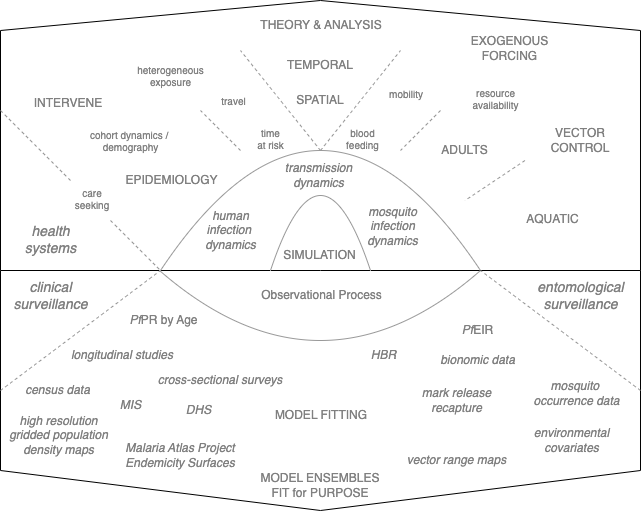
\includegraphics[width=0.8\textwidth,height=\textheight]{Figures/ScalableComplexity.png}
\caption{A schematic diagram of the elements in the framework (top half) and the process of model building and model fitting (bottom half)}
\end{figure}

This book has been written to introduce the features of the framework (see Figure 1.1). The book itself is embedded in the RAMP-Model-Library, which was set up during the primary design phase. The RAMP-Model-Library is where we made all our design mistakes: was the software truly plug-and-play, and was the framework truly extensible? As the primary design phase came to a close, the library that was once the laboratory became a classroom and a museum. The library is being transformed into a resource for any developer who wants to add new base models to the library or add functionality. Most of all, it is being set up for the end user, someone in a malaria program or working with a malaria program who wants to use simulation based analytics to analyze policies. This book is structured into a set of lessons that teach concepts. Some of the concepts build on one another, and others take on new challenges. We combine these lessons into some examples where we show some algorithms to build models fit for purpose. When a topic deserves a deeper dive, we have supplemented this book with vignettes or lessons.

In malaria epidemiology (narrowly defined as a study of infection and disease in humans), the relationship between exposure, infection, immunity, disease, and infectiousness changes in populations as they age, and it is affected by drug taking. This picture grows more complex as we consider intervening with vaccines or monoclonal antibodies, or as we look at interactions with anemia, nutritional status, and human genetics. Our models need to interface with data from clinical settings and research, so they will need to consider diagnostics, parasite counts, detection, and transmission. Combining these factors can give rise to an overwhelming amount of complexity. Later, we will introduce new models and show how it possible to simplify all this complexity and make sense of malaria.

We are interested in using these models to guide policy, which requires both solid computation and good communication. In this book, we lay a foundation for understanding the complexity by studying some simple compartmental models. We will review classical queuing models for superinfection and the multiplicity of infection (MoI); new models for the age of infection (AoI) or stage of infection (SoI); immunity; parasite densities, fever, disease, and detection; gametocytes and transmission, and drug taking. To end up with models that can handle all the complexity, we build probabilistic models that combine these factors. In doing so, we find that we can do some powerful analysis, and we can map the states in these models onto outcomes that matter for research and policy: test positivity, parasite counts, infectiousness, and disease. With patience, we can combine these factors and develop a framework for understanding malaria in populations that match the features of individual-based simulation models. We end up with a sensible understanding malaria epidemiology as ontogeny -- development of immunity as a part of an organisms history. We back this view with some very usable models that capture the changing character of malaria in cohorts of humans as they age.

We are interested in understanding malaria control in context, which requires delving into mosquito ecology and behavior. In this book, we start with a simple model for mosquito ecology and parasite infection dynamics in mosquitoes. We add aquatic population dynamics, mosquito population regulation, and exogenous forcing by weather. Later, we worry about adult mosquito behavioral states such as mating, sugar feeding, and egg laying. We introduce the concept of resource availability, and we develop an understanding of mosquito search and movement in response to resource availability. We take some deep dives to understand how mosquito spatial dynamics work at a fine spatial grain, and then we scale up to understand mosquito populations on landscapes.

At first, we describe mosquito blood feeding and transmission with a few simple parameters. Later, we develop a new model for mosquito blood feeding in a dynamically changing host population with parameters that allow host strata to be more or less available. We also modify our understanding of heterogeneous exposure to biting. We develop a methods for modeling environmental heterogeneity, heterogeneous exposure by age, and a generalized way of handling \href{Frailty}{failty}-- other sources of heterogeneous biting -- through stratification.

We must take a detour to understand how to handle the effects of temperature on the parasite's extrinsic incubation period (EIP). We need a way of dealing with mosquito survival and dispersal through the EIP. This problem has been effectively solved.

To round out this picture, we need a way of dealing with other aspects of human ecology that affect malaria transmission dynamics, including human mobility, human demography, bed net usage, adherance to drugs, and care seeking. Differences among humans call for a synthesis of studies that have identified traits that affect malaria, stratification, and simulation to identify useful ways of propagating the heterogeneity through analyses.

To go along with a theory of transmission, we need a theory of control. We compute effect sizes and evaluate area effects. We develop a generalized concept of effect modification that considers the total effect of a single unit of control. We modify basic processes by including the effects of vector control and mass medical interventions (\emph{e.g.} seasonal malaria chemoprotection, mass drug administration, vaccines, and monoclonal antibodies). Relying on behavioral state models and the concept of resource availability, we develop a models for integrated vector control.

\begin{center}\rule{0.5\linewidth}{0.5pt}\end{center}

In doing all this, we are building on an enormous body of work that started with Ronald Ross. While Ross is better known for identifying malaria parasites in a mosquito gut, which proved that malaria is mosquito transmitted, we are more interested in the academic work that followed.

After winning the Nobel Prize in 1902, Ross was instrumental in building solid quantitative foundations for malaria transmission and its measurement. Ronald Ross wrote the first models describing malaria transmission. In his writings from 1899 to 1908, it's clear that he was searching for quantitative way of saying something simple -- if there are not enough mosquitoes, the malaria transmission can't be sustained. There must be a critical mosquito density, above the cutoff malaria transmission would be sustained, and below it malaria would be eliminated. Ross was looking for a formula that encapsulated his intuition: how were thresholds related to the fact that it took two bites for a mosquito to complete its life cycle? Eventually, Ross wrote down some systems of equations that would describe malaria. The ideas, mathematics, and identification of parameters and processes were extended by other scientists later, most notably Alfred Lotka and George Macdonald.

It seems that the challenge of malaria control was what pushed Ross toward modeling. Ross's first model was a discussion of adult mosquito movement to guide larval source management {[}\protect\hyperlink{ref-RossR1905LogicalBasis}{10}{]}. The first model describing malaria transmission appeared in a book, \emph{The Prevention of Malaria in Mauritius} {[}\protect\hyperlink{ref-RossR1908ReportPrevention}{11}{]}. When it came to thinking through control, Ross found it useful to do the math.

\begin{center}\rule{0.5\linewidth}{0.5pt}\end{center}

This is a book about how to do the math that is required for malaria programs. The goal is to use all the data available, but especially the data generated by malaria programs, to paint a clear picture of malaria transmission as a changing baseline that has been modified by control. The software is structured into three major domains: the humans and malaria epidemiology, including the effects of treating malaria with drugs; the mosquitoes and the way they have been changed by weather and vector control; and parasite transmission through mosquito blood feeding. Within each domain, there are multiple sub-domains, and there are built in design features to deal with heterogeneity and other features for malaria control. After a 140 years of studying malaria, there's a lot of detail that could be important in some way. Part of what we need to do is sort through all that detail to find what is most relevant.

We have organized the concepts in this book around a narrative that allows us to introduce the core concepts -- those that make modular computation possible -- in an order that minimizes the need to draw on unfamiliar concepts. We start with the Ross-Maconald model, but our next task is to update the model for mosquito blood feeding.

Our philosophy has been to design a framework for model building that can be used by programs. The material in this book is designed to be used by non-experts too, so in this context, \emph{model building} means applying a set of tools to to computational tasks we wish our brains could do.

The software we have developed is meant to lower the costs of building and using models. We want programs to be focused on the decisions, the data, the concepts, and the analysis. As a metaphor, some students learn a numerical method for approximating \(\sqrt{2}\) in school, but after learning it once, they stop worrying about \emph{how} it is computed and they punch buttons into a calculator. Knowing how to compute something is sometimes useful, but worrying about how to compute it each time would interrupt the process that called for computing it. Instead, we punch the formula into a scientific calculator or any software that does computation confident that the machine knows how to do it. In applying models, the same kind of logic applies. People need to understand the concepts, but like a calculator, the tools should hide the technical details that don't add to a discussion. The software we have developed is a reliable interface for calculations designed to support policy.

To learn how to use that software, we need to get through a lot of material. The background material in the following presentation is fairly sparse. We are trying to introduce just \emph{enough} mathematics to teach users the critical concepts so they know what the software can do. We assume that the work will be done by teams that include a few people who understand the mathematics, who can guide others through the process. To fill in some of the gaps and technical, we have written (or can write) vignettes. On occasion, the text includes links to these vignettes for those who might find them useful. Please send suggestions about new vignettes to \href{mailto:smitdave@gmail.com}{\nolinkurl{smitdave@gmail.com}}.

The first model we present is a Ross-Macdonald model.

\hypertarget{contributors}{%
\section*{Contributors}\label{contributors}}
\addcontentsline{toc}{section}{Contributors}

This is a work in progress, so the list of contributors will change over time.

The software package \texttt{MicroMoB} was written by Sean L Wu, Sophie Liebkind, and David L Smith. The software package \texttt{exDE} was written by Sean L Wu and David L Smith.

Most of the content so far was written by David L Smith. Contributors from the RAMP Team include:

\begin{itemize}
\tightlist
\item
  \ldots please consult Dave if you would like a writing role.
\end{itemize}

\textbf{David L. Smith}

\hypertarget{part-basic-concepts}{%
\part{Basic Concepts}\label{part-basic-concepts}}

\hypertarget{malaria-dynamics}{%
\chapter{Malaria Dynamics}\label{malaria-dynamics}}

We start by introducing a Ross-Macdonald model {[}\protect\hyperlink{ref-SmithDL2012_RossMacdonald}{1}{]}. This particular model family is a system of delay differential equations that traces back to a 1982 book chapter written by Joan Aron and Robert May {[}\protect\hyperlink{ref-AronJL1982PopulationDynamics}{12}{]}. We think it's a good starting point.

We chose it because it is \emph{extensible}. The variables represent population densities, which are used to compute proportions, like \emph{prevalence.} The variables in many other versions of the Ross-Macdonald are proportions. In some models, we would like to be able to change the \emph{total} number of hosts, but if the variables are proporions, these are the denominators. When a variables in equations described proportions, they are much more difficult to modify.

We chose it because it already includes mosquito ecology, so we can bypass a lengthy discussion of the limitations of the Ross-Macdonald model. While Macdonald's analysis and formulas are familiar, they were not complete {[}\protect\hyperlink{ref-SmithDL2004_Statics}{13},\protect\hyperlink{ref-SmithDL2021_NewTestOldMosquitoes}{14}{]}. We develop a formula for vectorial capacity that is consistent with the intent of the original, but our analysis of sensitivity to parameters includes effects on mosquito ecology {[}\protect\hyperlink{ref-BradyOJ2015AdultVector}{15}{]}. (A lengthy and philosophical discussion of the history and its failings is planned.)

We chose it because it is \emph{realistic.} Time does not appear in most versions of the Ross-Macdonald model: the equations are \emph{autonomous}. These equations use time to drive a seasonal pattern: they are \emph{non-autonomous}. Since we know we are interested in dealing with exogenous forcing, we start out with a model that is forced.

While the following model is basic, we recommend reading it, if only because we introduce concepts and conventions that are important for the software design.

\hypertarget{aron-and-mays-equations}{%
\section{Aron and May's Equations}\label{aron-and-mays-equations}}

The simplest quantitative description of malaria dynamics tracks the number of infected and infectious mosquitoes and the number of infected and infectious humans. To develop systems of equations, we assign names to variables that represent these quantities: the number of infected and infectious people is denoted \(X(t)\) (out of \(H\) total); the number of mosquitoes is \(M(t)\); the number of infected mosquitoes is \(Y(t)\) (out of \(M(t)\) total); and the number of infectious mosquitoes is denoted \(Z(t)\) (out of \(M(t)\) total).

In dynamical systems, we ask how the variables (\emph{i.e.} \(M\), \(Y\), \(Z\), and \(X\)) change over time. For our first equation, we start with adult, female mosquito populations. (It is tiresome to repeat \emph{adult, female} each time, and we're ignoring male mosquitoes at this point anyway, so \emph{mosquito} hereafter means \emph{adult, female mosquito}, unless we say otherwise.) The number of mosquitoes is changing as new adults emerge from aquatic habitats or die.

\hypertarget{mosquito-ecology}{%
\subsection{Mosquito Ecology}\label{mosquito-ecology}}

To model changes in \(M\), we assume the following:

\begin{itemize}
\item
  mosquitoes emerge from aquatic habitats at the rate of \(\Lambda(t)\) adults, per day;
\item
  mosquitoes die at a constant rate, \(g\). This is equivalent to assuming that the mosquito lifespan is exponentially distributed with a mean \(1/g\). The fraction surviving one day is \(e^{-g}\).
\end{itemize}

Our first equation describes changes in the number of mosquitoes:

\begin{equation}
\frac{dM}{dt} = \Lambda(t) - g M
\end{equation}

\hypertarget{blood-fed-mosquitoes}{%
\subsection{Blood Fed Mosquitoes}\label{blood-fed-mosquitoes}}

At this point, we will take a detour and define a variable describing the density of mosquitoes that have blood fed at least once, \(V\). After blood feeding, a mosquito is either gravid or \emph{parous}, meaning its ovaries are distended from laying an egg batch. We do this, in part, because the fraction of mosquitoes that are parous is routinely collected, and because it gives us a chance to focus on blood feeding.

To describe \emph{blood feeding}, we assume the following:

\begin{itemize}
\item
  mosquitoes blood feed at the rate \(f\), per mosquito, per day; in this model, this implies that the waiting time to a blood meal is \(1/f\) days.
\item
  a fraction of all mosquito blood meals, \(q\), is taken on humans; we call this the \emph{human fraction}
\item
  the human blood feeding rate is the product of these two parameters, \(fq\), which is defined as the number of human blood meals, per mosquito, per day.
\end{itemize}

The number of human blood meals by a population of vector mosquitoes, per person, per day is called the human biting rate (HBR). In this model, HBR is given by a formula:

\[\mbox{HBR} = \frac{fqM}{H}\]

Later, we discuss the correspondence between the HBR in models and data.

\begin{equation}
\frac{dV}{dt} = f q (M-V) - g V
\end{equation}

We won't use \(V\) to describe the dynamics of infection, but we might find it useful to understand how parity changes in mosquito populations.

\hypertarget{infected-mosquitoes}{%
\subsection{Infected Mosquitoes}\label{infected-mosquitoes}}

Mosquitoes become infected after blood feeding on an infectious human. To model changes in \(Y\), we extend the model of blood feeding to include infection. We need to know what fraction of blood meals end up infecting a mosquito that has not already been infected.

To model changes in \(Y\), we need to describe \emph{infection rates}. We assume the following:

\begin{itemize}
\tightlist
\item
  a fraction of human blood meals, infects mosquitoes. We call this quantity \emph{net infectiousness} (NI) and (for reasons that we will discuss in a moment), we give it a name, \(\kappa\):
\end{itemize}

\begin{equation}
\kappa(t) = c \frac{X(t)}{H}
\label{eq:kappaDef}
\end{equation}

\begin{itemize}
\tightlist
\item
  infected mosquitoes die at the same rate as uninfected mosquitoes.
\end{itemize}

We can now write down our second equation describing changes in the number of infected mosquitoes:

\begin{equation}
\frac{dY}{dt} = f q \kappa (M-Y) -g Y
\end{equation}

\hypertarget{infectious-mosquitoes}{%
\subsection{Infectious Mosquitoes}\label{infectious-mosquitoes}}

To become infectious, a mosquito has to become infected and then survive through the extrinsic incubation period (EIP). We assume:

\begin{itemize}
\item
  mosquitoes become infectious after a fixed delay, \(\tau\) days, called the EIP. The fraction of mosquitoes that survive through the EIP is \(e^{-g \tau}\).
\item
  infectious mosquitoes die at the same rate as other mosquitoes.
\end{itemize}

For a mosquito to become infectious, it must have become infected \(\tau\) days ago and survived through \(\tau\) days with probability \(e^{-g\tau}\). To write this in equations, we use a subscripted \(\tau\) to denote the value of a variable (\(M\), \(Y\) or \(X\)) or term (\(\kappa\)) at time \(t-\tau\). For example \(X_\tau\) is the number of people who were infected and infecious at time \(t-\tau\), and \(M_\tau\) is the number of mosquitoes at time \(t-\tau\).

The number of infectious mosquitoes that are added to the population at a point in time includes all the mosquitoes that became infected at time \(t-\tau\) and survived the EIP. This is our third equation describing changes in the number of infectious mosquitoes:

\begin{equation}
\frac{dZ}{dt} = f q  \kappa_\tau (M_\tau-Y_\tau) e^{-g\tau} -g Z
\end{equation}

Here, \(Z\) represents the number of mosquitoes with \emph{sporozoites} in their salivary glands. The \emph{fraction} of mosquitoes with sporozoites in their salivary glands has been called the \emph{sporozoite rate} (SR), which in our notation is

\[ z = \frac{Z}{M}\]

The number of bites by vector mosquitoes, per person, per day is called the entomological inoculation rate (EIR). It is defined as the product of the HBR and the SR:

\[\mbox{EIR} = \mbox{SR} \times \mbox{HBR}\]

In our notation, the EIR is:

\[\mbox{EIR} = z \frac{fqM}{H} = \frac{fqZ}{H}\]
As with the HBR, we would like to know how to connect estiamted values of the EIR to our formulas. Since that's \emph{really} complicated, we've spent a lot of time in the following sections discussing it.

\hypertarget{RossEqn}{%
\subsection{Infected Humans}\label{RossEqn}}

Humans become infected after being bitten by an infectious mosquito. We assume the following:

\begin{itemize}
\item
  A fraction \(b\) of all bites by infectious mosquitoes cause an infection.
\item
  The hazard rate for infection, also called the \emph{force of infection} (FoI) and denoted \(h\) is \(b \times\) EIR: \[h = fqb \frac{Z}{H}\]
\item
  Infections clear at the rate \(r\), per infection, per day (the average time to clear is \(1/r\) days), and after clearing an infection a person becomes susceptible to infection again.
\end{itemize}

We can now write down our fourth equation describing changes in the number of infected humans:

\begin{equation}
\frac{dX}{dt} = h (H-X) - r X 
\end{equation}

\hypertarget{as-a-system}{%
\subsection{\ldots as a System}\label{as-a-system}}

While we presented these equations one at a time, they work as a system. To see it all at once, we write it here as a system with four equations and two terms:

\begin{equation}
\begin{array}{rl}
\frac{dM}{dt} &= \Lambda(t) - g M \\
\frac{dY}{dt} &= fq\kappa(M-Y) - g Y \\
\frac{dZ}{dt} &= fq\kappa_\tau(M_\tau-Y_\tau)e^{-g\tau} - g Z \\
\frac{dX}{dt} &= h (H-X) - rX  \\ \\ \hline \\ 
\kappa &= c \frac{X(t)}{H} \\
h &= b fq \frac{Z(t)}{H} \\
\end{array}
\end{equation}

\begin{figure}
\centering
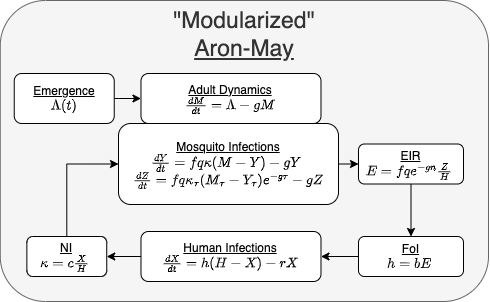
\includegraphics{Figures/AronMay.png}
\caption{A diagram of the a version of the Ross-Macdonald model, using equations from Aron and May {[}\protect\hyperlink{ref-AronJL1982PopulationDynamics}{12}{]}}
\end{figure}

These equations describe processes in three domains (Figure 2.1):

\begin{itemize}
\item
  adult mosquito ecology (\(M\), and perhaps \(V\));
\item
  parasite infection dynamics in mosquito populations (\(Y\) and \(Z\));
\item
  parasite infection dynamics in human populations (\(X\)).
\end{itemize}

The equations describing parasite infections in mosquito populations also include the variable \(M\), so the mosquito infection dynamics are coupled to the mosquito population dynamics. The way we've written the equations, each compartment has an input term (\emph{i.e.}, \(\Lambda\), \(\kappa\), or \(h\)) that depends on something else. We've passed \(\Lambda\) as a parameter. For the infection dynamics, the terms \(\kappa\) and \(h\) couple two separate systems. For adult mosquito dynamics, emergence is passed to the model as a parameters.

There are, of course, more compact ways of writing these equations. We have written the equations this way to emphasize a few things. First, the terms make it clear exactly how the equations in one domain are connected to another. Second, if we wanted to start \emph{changing} some of the assumptions, these terms help to isolate the parts we might like to change. By writing the equations in this modularized form, we can start to understand how we might be able to write software that would allow us to represent mosquito infection dynamics with different systems of equations.

The next step is to find solutions.

\emph{NOTE:} We don't introduce \texttt{exDE} or \texttt{MicroMoB} until {[}Modularity and Software{]}.

\hypertarget{solutions}{%
\section{Solutions}\label{solutions}}

What does a \textbf{solution} to these equations look like?

Solutions to these equations are values of the variables over time \(\left( M(t), Y(t), Z(t), X(t) \right)\) that satisfy the system of four equations described above. We call these solutions \emph{orbits.} To put it another way, if we took the derivatives of the orbits for any variable at any point in time using the basic definition \[\lim_{h\rightarrow 0} \frac{x(t+h)-x(t)}{h},\] and then we used the values of the variables at time \(t\) to compute \(dM/dt\), \(dY/dt\), \(dZ/dt\), and \(dX/dt\) (\emph{i.e.}, using the formulas), we would get the same values.

It is important that these orbits are unique: after specifying the \emph{initial values} of the variables, there is one and only one set of orbits that solves the equations. When we solve the equations, we usually produce solutions from a starting point into a future, but the orbits are defined for all time -- \(i.e.\) the process implies the existence of solutions far back into the past. These are deterministic equations, after all.

As written, the equations do not define a \emph{model.} Instead, the equations define a process or a \textbf{model family.} A model is something that \emph{can} produce orbits. A model is defined only after assigning specific values to the parameters. Informally, we will often slip and use the ``model'' to describe a model family. It's easy to slip up, and sometimes we can get by with being sloppy, but we need to remember the distinction. When we say that the software is \emph{modular,} we mean that it is easy to swap out one \emph{model family} for another.

To find solutions of equations we use an R software package called \texttt{deSolve.} Because of the delay for the EIP, these are called \emph{delay differential equations,} which are handled using a function called \texttt{dede}. An important step in solving delay differential equations is a function \texttt{lagvalue()} that computes and returns the values of variables at a time lag, \(\ell\). In these equations, the lag is set by the EIP, \(\tau\), so we must evaluate
\texttt{lagvalue(t-tau).}

In solving \emph{ordinary differential equations,} we must pass initial conditions. To solve a delay differential equations with a maximum lag \(\ell\), we must specify the initial conditions for the interval \([-\ell, t_0)\), where \(t_0\) is the point in time when we start computing solutions.
In these equations, since the equation for \(dZ/dt\) looks back \(\tau\) units, we must specify values of \(M(t)\), \(Y(t)\), and \(X(t)\) for all values of \(t \in [-\tau, t_0)\). This forces an awkward choice, since we don't know the solutions backwards in time, but would need to know those solutions to use them. What is typically done -- and we've done it here -- is to specify a constant set of initial values and moving on.

Doing this introduces a little \emph{numerical slop.} By slop, we mean that these values are \emph{not} what we would get if we ran the equations backwards in time. In these equations, it won't affect our analysis most of the time, so we're happy to acknowledge this little problem and find ways around it. It's a little thing, but we should never forget it, because we might find that it \emph{is} affecting our analysis at some point.

With \texttt{deSolve,} solving differential equations is not difficult -- it just involves following a few steps. In the following, we walk through these steps:

\begin{itemize}
\item
  Write a function that computes the derivatives;
\item
  Define initial conditions;
\item
  Define the values of the parameters;
\item
  Define a mesh on time;
\item
  Call a function that solves the equations, such as \texttt{dede} for delay differential equations.
\end{itemize}

Many users will find that reading this code is like learning how to compute \(\sqrt{2}\). If so, feel free to learn it once and then skip it.

\hypertarget{derivatives}{%
\subsection{Derivatives}\label{derivatives}}

The first step is to write down the equations to compute the derivatives. The solver expects a function with three required arguments (in this order):

\begin{itemize}
\item
  \texttt{t} is time
\item
  \texttt{y} is the list of variables
\item
  \texttt{params} is a set of parameters
\end{itemize}

The derivatives are computed and returned in the same order as `y' in a \texttt{list}. To make code that is easy to read, we make \texttt{params} as a \texttt{list} with parameter names (see below), so that inside the function \texttt{with(params,\{...\})}, the parameter names are visible.

\begin{Shaded}
\begin{Highlighting}[]
\NormalTok{dAronMay }\OtherTok{=} \ControlFlowTok{function}\NormalTok{(t, y, params)\{}\FunctionTok{with}\NormalTok{(params,\{}
 
  \CommentTok{\# Variables  }
  \ControlFlowTok{if}\NormalTok{(t}\SpecialCharTok{\textless{}=}\NormalTok{tau) ylag}\OtherTok{\textless{}{-}}\NormalTok{y0 }\ControlFlowTok{else}\NormalTok{ ylag }\OtherTok{\textless{}{-}} \FunctionTok{lagvalue}\NormalTok{(t}\SpecialCharTok{{-}}\NormalTok{tau)}
\NormalTok{  M}\OtherTok{=}\NormalTok{y[}\DecValTok{1}\NormalTok{]; M\_tau }\OtherTok{=}\NormalTok{ ylag[}\DecValTok{1}\NormalTok{]}
\NormalTok{  Y}\OtherTok{=}\NormalTok{y[}\DecValTok{2}\NormalTok{]; Y\_tau }\OtherTok{=}\NormalTok{ ylag[}\DecValTok{2}\NormalTok{]; }
\NormalTok{  Z}\OtherTok{=}\NormalTok{y[}\DecValTok{3}\NormalTok{]; }
\NormalTok{  X}\OtherTok{=}\NormalTok{y[}\DecValTok{4}\NormalTok{]; X\_tau }\OtherTok{=}\NormalTok{ ylag[}\DecValTok{4}\NormalTok{]}
   
  \CommentTok{\# Terms }
\NormalTok{  kappa }\OtherTok{=}\NormalTok{ c}\SpecialCharTok{*}\NormalTok{X}\SpecialCharTok{/}\NormalTok{H; kappa\_tau }\OtherTok{=}\NormalTok{ c}\SpecialCharTok{*}\NormalTok{X\_tau}\SpecialCharTok{/}\NormalTok{H}
\NormalTok{  h }\OtherTok{=}\NormalTok{ b}\SpecialCharTok{*}\NormalTok{f}\SpecialCharTok{*}\NormalTok{q}\SpecialCharTok{*}\NormalTok{Z}\SpecialCharTok{/}\NormalTok{H }
   
  \CommentTok{\# Dynamics }
\NormalTok{  dM }\OtherTok{=} \FunctionTok{Lambda}\NormalTok{(t) }\SpecialCharTok{{-}}\NormalTok{ g}\SpecialCharTok{*}\NormalTok{M}
\NormalTok{  dY }\OtherTok{=}\NormalTok{ f}\SpecialCharTok{*}\NormalTok{q}\SpecialCharTok{*}\NormalTok{kappa}\SpecialCharTok{*}\NormalTok{(M}\SpecialCharTok{{-}}\NormalTok{Y) }\SpecialCharTok{{-}}\NormalTok{g}\SpecialCharTok{*}\NormalTok{Y}
\NormalTok{  dZ }\OtherTok{=}\NormalTok{ f}\SpecialCharTok{*}\NormalTok{q}\SpecialCharTok{*}\NormalTok{kappa\_tau}\SpecialCharTok{*}\NormalTok{(M\_tau}\SpecialCharTok{{-}}\NormalTok{Y\_tau)}\SpecialCharTok{*}\FunctionTok{exp}\NormalTok{(}\SpecialCharTok{{-}}\NormalTok{g}\SpecialCharTok{*}\NormalTok{tau) }\SpecialCharTok{{-}}\NormalTok{g}\SpecialCharTok{*}\NormalTok{Z}
\NormalTok{  dX }\OtherTok{=}\NormalTok{ h}\SpecialCharTok{*}\NormalTok{(H}\SpecialCharTok{{-}}\NormalTok{X)}\SpecialCharTok{{-}}\NormalTok{r}\SpecialCharTok{*}\NormalTok{X}
  
  \FunctionTok{return}\NormalTok{(}\FunctionTok{list}\NormalTok{(}\FunctionTok{c}\NormalTok{(dM, dY, dZ, dX)))}
\NormalTok{\})\} }
\end{Highlighting}
\end{Shaded}

\hypertarget{initial-values}{%
\subsection{Initial Values}\label{initial-values}}

To run the model, we must supply initial values. If you were writing code yourself, it would be important to remember that the initial values and the return value for the derivatives must occur in the same order.

A useful convention in \{R\} is to pass the initial values as a named list. Later, we can turn the outputs into a data frame, and then we can retrieve the variables by name.

\begin{Shaded}
\begin{Highlighting}[]
\NormalTok{y0}\OtherTok{=} \FunctionTok{c}\NormalTok{(}\AttributeTok{M=}\DecValTok{60}\NormalTok{, }\AttributeTok{Y=}\DecValTok{0}\NormalTok{, }\AttributeTok{Z=}\DecValTok{0}\NormalTok{, }\AttributeTok{X=}\DecValTok{1}\NormalTok{)}
\end{Highlighting}
\end{Shaded}

The object \texttt{y0} is a named list -- the names are attached but invisible.

\begin{Shaded}
\begin{Highlighting}[]
\NormalTok{y0}
\end{Highlighting}
\end{Shaded}

\begin{verbatim}
##  M  Y  Z  X 
## 60  0  0  1
\end{verbatim}

When we turn it into a list, with \texttt{as.list,} the names are attached to the values:

\begin{Shaded}
\begin{Highlighting}[]
\FunctionTok{as.list}\NormalTok{(y0)}\SpecialCharTok{$}\NormalTok{M}
\end{Highlighting}
\end{Shaded}

\begin{verbatim}
## [1] 60
\end{verbatim}

If we use \texttt{with}, we create an environment where we can simply use the names:

\begin{Shaded}
\begin{Highlighting}[]
\FunctionTok{with}\NormalTok{(}\FunctionTok{as.list}\NormalTok{(y0), \{}
\NormalTok{  M}
\NormalTok{\})}
\end{Highlighting}
\end{Shaded}

\begin{verbatim}
## [1] 60
\end{verbatim}

\hypertarget{parameter-values}{%
\subsection{Parameter Values}\label{parameter-values}}

We pass the parameters as a list. It might seem like overkill, but we have written a function \texttt{makeParams()} that takes default values and generates a list. This makes it easy to generate a new set of parameter values with alternative values, and it also helps us to write and pass function \(\Lambda(t)\) with parameters we like. By passing the parameter as a list, the parameter values are available to the function \texttt{dAronMay} when we use \texttt{with(params,\ \{\})}.

Note that we have also attached the initial values of the variables as a parameter set, which are the return values for \texttt{lagvalue(t)} when \texttt{t\textless{}0}.

\begin{Shaded}
\begin{Highlighting}[]
\NormalTok{makeParams }\OtherTok{=} \ControlFlowTok{function}\NormalTok{(y0, }
                      \AttributeTok{g=}\DecValTok{1}\SpecialCharTok{/}\DecValTok{12}\NormalTok{, }\AttributeTok{f=}\DecValTok{1}\SpecialCharTok{/}\FloatTok{2.5}\NormalTok{, }\AttributeTok{q=}\FloatTok{0.95}\NormalTok{,  }
                      \AttributeTok{c=}\FloatTok{0.15}\NormalTok{,}
                      \AttributeTok{b=}\FloatTok{0.55}\NormalTok{, }\AttributeTok{r=}\DecValTok{1}\SpecialCharTok{/}\DecValTok{200}\NormalTok{, }\AttributeTok{H=}\DecValTok{1000}\NormalTok{,  }
                      \AttributeTok{m=}\NormalTok{.}\DecValTok{05}\NormalTok{, }\AttributeTok{ss=}\DecValTok{1}\NormalTok{,  }
                      \AttributeTok{tau=}\DecValTok{10}  
\NormalTok{                      )\{}
\NormalTok{  ss }\OtherTok{=} \FunctionTok{min}\NormalTok{(}\DecValTok{1}\NormalTok{,}\FunctionTok{max}\NormalTok{(}\DecValTok{0}\NormalTok{, ss))}
\NormalTok{  Lambda }\OtherTok{=} \ControlFlowTok{function}\NormalTok{(t)\{m}\SpecialCharTok{*}\NormalTok{H}\SpecialCharTok{*}\NormalTok{(}\DecValTok{1} \SpecialCharTok{+}\NormalTok{ ss}\SpecialCharTok{*}\FunctionTok{sin}\NormalTok{(}\DecValTok{2}\SpecialCharTok{*}\NormalTok{pi}\SpecialCharTok{*}\NormalTok{t}\SpecialCharTok{/}\DecValTok{365}\NormalTok{))\}}
  \FunctionTok{return}\NormalTok{(}\FunctionTok{list}\NormalTok{(}\AttributeTok{y0=}\NormalTok{y0,}\AttributeTok{g=}\NormalTok{g,}\AttributeTok{f=}\NormalTok{f,}\AttributeTok{q=}\NormalTok{q,}\AttributeTok{c=}\NormalTok{c,}
              \AttributeTok{H=}\NormalTok{H,}\AttributeTok{m=}\NormalTok{m,}\AttributeTok{tau=}\NormalTok{tau,}\AttributeTok{b=}\NormalTok{b,}\AttributeTok{r=}\NormalTok{r,}\AttributeTok{Lambda=}\NormalTok{Lambda))}
\NormalTok{\} }
\NormalTok{params }\OtherTok{=} \FunctionTok{makeParams}\NormalTok{(y0)}
\end{Highlighting}
\end{Shaded}

To make it absolutely clear, we are assuming:

\begin{itemize}
\item
  \(g=1/12\): mosquitoes live about \(12\) days, on average
\item
  \(f=1/2.5\): mosquitoes feed every 2.5 days, on average
\item
  \(q=0.95\): the human fraction is 95\%; mosquitoes feed on humans 95\% of the time
\item
  \(c=0.15\): about 15\% of bites on infectious humans infect a mosquito
\item
  \(b=0.55\): about 55\% of bites by infective mosquitoes cause an infection
\item
  \(r=1/200\): human infections last about \(200\) days, on average
\item
  \(H=1000\): we're simulating transmission in a population of a thousand humans
\item
  \(\tau=10\): the extrinsic incubation period is about 10 days
\item
  For emergence, we tune the average value using \(m\) and it is scaled to \(H\):

  \begin{itemize}
  \item
    The parameter \(m\) in the function above has been set to \(0.05\) by default.
  \item
    The parameter \(ss\) affects the amplitude of the fluctuations. We force it to take on values between 0 and 1.
  \item
    Emergence is modeled as a sinusoidal function with a yearly cycle.
  \end{itemize}
\end{itemize}

\[\Lambda(t) = m H \left(1 + \sin \left(\frac{2\pi t}{365}\right)\right)\]

\hypertarget{solving}{%
\subsection{Solving}\label{solving}}

We define a mesh over time -- the points in time when we would like to know the values of the variables:

\begin{Shaded}
\begin{Highlighting}[]
\NormalTok{tt }\OtherTok{=} \FunctionTok{seq}\NormalTok{(}\DecValTok{0}\NormalTok{,}\DecValTok{5}\SpecialCharTok{*}\DecValTok{365}\NormalTok{, }\AttributeTok{by=}\DecValTok{5}\NormalTok{) }
\end{Highlighting}
\end{Shaded}

This code solves the equations:

\begin{Shaded}
\begin{Highlighting}[]
\FunctionTok{require}\NormalTok{(deSolve)}
\NormalTok{yout }\OtherTok{\textless{}{-}} \FunctionTok{dede}\NormalTok{(}\AttributeTok{y=}\NormalTok{y0, }\AttributeTok{times=}\NormalTok{tt, }\AttributeTok{func=}\NormalTok{dAronMay, }\AttributeTok{parms=}\NormalTok{params) }
\end{Highlighting}
\end{Shaded}

\hypertarget{visualizing}{%
\subsection{Visualizing}\label{visualizing}}

When we plot out the solutions, they look like this.

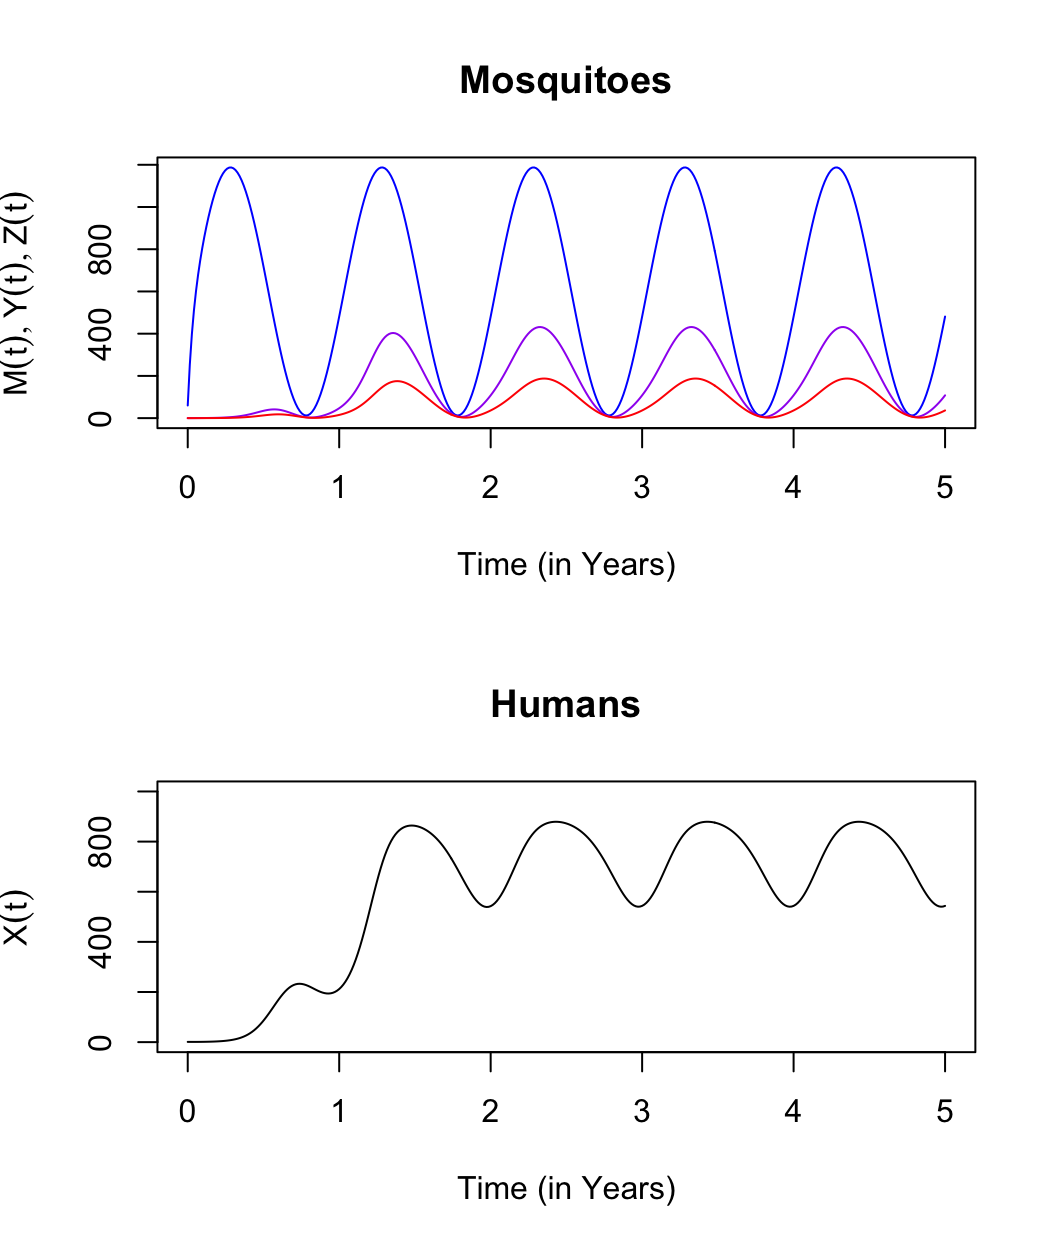
\includegraphics{_main_files/figure-latex/unnamed-chunk-10-1.pdf}

\clearpage

\hypertarget{steady-states}{%
\section{Steady States}\label{steady-states}}

Here, we analyze the system of equations in a narrow case when there is \emph{no seasonality,} and the system reaches a \emph{steady state.} To do so, we set the parameter \texttt{ss=1}, so that \(\Lambda(t)\) is a constant; the resulting system is \emph{autonomous.} We do this, in part, because the resulting system is easier to understand. We can develop intuition that can be applied (albeit with caution) to more complex systems. To be clear, we are dealing with this system:

\begin{equation}
\begin{array}{rl}
\frac{dM}{dt} &= \Lambda - g M \\
\frac{dY}{dt} &= fq\kappa(M-Y) - g Y \\
\frac{dZ}{dt} &= fq\kappa_\tau(M_\tau-Y_\tau)e^{-g\tau} - g Z \\
\frac{dX}{dt} &= h (H-X) - rX  \\ \\ \hline \\ 
\kappa &= c \frac{X(t)}{H} \\
h &= b fq \frac{Z(t)}{H} \\
\end{array}
\end{equation}

As before, we have put the equations in their modularized form above, and the connecting terms below.

The first thing to note is that \(M\) affects \(Y\) and \(Z\), which affect \(X\); but \(M\) is not affected by \(Y\) or \(Z\). Mosquito population density is \emph{exogenous} to malaria dynamics.

\hypertarget{mosquito-density}{%
\subsection{Mosquito Density}\label{mosquito-density}}

We can thus treat it separately in the analysis:

\begin{equation}
\frac{dM}{dt} = \Lambda - g M 
\end{equation}

Since emergence rates are steady, mosquito population density reaches a steady state when \(dM/dt=0\), which occurs at:

\begin{equation}
\bar M = \frac{\Lambda}{g} 
\end{equation}

\hypertarget{eir}{%
\subsection{EIR}\label{eir}}

Next, we note that at a steady state, the delayed values of variables and terms don't change, so from \(dY/dt\), we get:

\begin{equation}
g \bar Y = fq\kappa(\bar M- \bar Y) 
\end{equation}

If we substitute the formula for \(\bar M\) and solve for \(\bar Y\), we get:

\begin{equation}
\bar Y = \frac{fq\kappa}{g + fq\kappa} \frac{\Lambda}{g}
\end{equation}

and since at the steady state, any variable at time \(t+\tau\) is equal to its value at time \(t\), we substitute the formula for \(g \bar Y\) into \(dZ/dt\) to get:

\begin{equation}
g \bar Y e^{-g\tau} = g \bar Z
\end{equation}

Solving for \(\bar Z\) we get:

\begin{equation}
\bar Z =  \frac{f q \kappa}{g + fq \kappa} \frac{\Lambda}{g} e^{-g\tau} 
\end{equation}

At the steady state, \[\mbox{EIR} = fq \frac{\bar Z}{H}.\]

In field studies, the EIR is the product of the HBR and the sporozoite rate (SR). The sporozoite rate (SR, \(z\)) is given by:

\begin{equation}
\bar z =  \frac{Z}{M} = \frac{f q \kappa}{g + fq \kappa} e^{-g\tau} 
\end{equation}

So we can understand the EIR as having two parts:

\begin{equation}
\mbox{EIR} = \mbox{HBR} \times  \mbox{SR} 
\end{equation}

or equivalently

\begin{equation}
\mbox{EIR} = \frac{\textstyle{fq\Lambda}}{\textstyle{H}} \times \frac{\textstyle{f q \kappa}}{\textstyle{g + fq \kappa}} e^{-g\tau} 
\end{equation}

This formula for the SR (albeit with slightly different notation) was originally derived as part of the Ross-Macdonald model {[}\protect\hyperlink{ref-MacdonaldG1952_SporozoiteRate}{16},\protect\hyperlink{ref-ArmitageP1953NoteEpidemiology}{\textbf{ArmitageP1953NoteEpidemiology?}}{]}. Also, Smith and McKenzie (2004) have written a useful discussion of mosquito demography {[}\protect\hyperlink{ref-SmithDL2004_Statics}{13}{]}.

\hypertarget{vectorial-capacity}{%
\subsection{Vectorial Capacity}\label{vectorial-capacity}}

Here, we pause to define a term that describes the number of human blood meals each mosquito would take over its whole life:

\[S = \frac{fq}{g}.\]

Since \(1/g\) is the mosquito lifespan in days, and \(fq\) is the human blood feeding rate, \(S\) is the number of human bloodmeals a mosquito would take over its lifespan. Intuitively, it makes sense that this \emph{should} be what drives transmission, since it takes two human blood meals to transmit malaria parasites.

If we rearrange the terms a bit, we can rewrite out the expression for the EIR:

\begin{equation}
\mbox{EIR}(\kappa) = fq \frac{\bar Z}{H} = \frac{\Lambda}{H} S^2  e^{-g\tau} \frac{\kappa}{1 + S \kappa} 
\end{equation}

This formula for the EIR has two parts. We call the first part \emph{vectorial capacity} (\(V\)):

\begin{equation}
V = \frac{\Lambda}{H} S^2  e^{-g\tau} 
\label{eq:VCdefined}
\end{equation}

The second part is an expression that involves mainly \(\kappa\).

\begin{equation}
\frac{\kappa}{1 + S \kappa} 
\label{eq:EIR2ndpart}
\end{equation}

The relationship between VC and EIR at a steady state is a product:

\begin{equation}
\mbox{EIR}(\kappa) = V \frac{\kappa}{1 + S \kappa} 
\label{eq:EIR2VC}
\end{equation}

Vectorial capacity describes the slope of the EIR when \(\kappa\) is small:

\begin{equation}
\left. d\frac{\mbox{EIR}(\kappa)}{d\kappa}\right|_{\kappa = 0} = V
\label{eq:VCisdEIR}
\end{equation}

We say that VC describes \emph{potential} transmission, even if the parasites are absent. Another way to say the same thing is that when \(\kappa\) is small, then:

\begin{equation}
\mbox{EIR}(\kappa) \approx V \kappa
\end{equation}

We can interpret vectorial capacity (\(V\)) in simple terms. It describes \emph{the number of infective bites that would arise from all the mosquitoes biting a single human on a single day} but only \emph{if all those mosquitoes became infected.} Vectorial capacity tells the story of potential parasite transmission by mosquitoes in four steps, which highlights the fact that two human blood meals are required for the parasite to be transmitted and complete its life-cycle.

\begin{equation}
\begin{array}{|c|c|c|c|c|c|c|}
\Lambda/H &  & S \kappa &  & e^{-g\tau} & & S \\
& \rightarrow &  & \rightarrow &  & \rightarrow &  \\
\mbox{Mosquito} & & \mbox{Parasite} & & \mbox{Mosquito} && \mbox{Parasite} \\
\mbox{Emerges} & & \mbox{Infects} & & \mbox{Survives} && \mbox{Infects} \\
 & & \mbox{Mosquito} & & \mbox{EIP} && \mbox{Human}
\end{array}
\label{eq:VCstory}
\end{equation}

As a reminder, while Eq. \eqref{eq:VCstory} includes \(\kappa\), the formula for VC, in Eq. \eqref{eq:VCdefined}, assumes that \(\kappa=1\): the VC describes transmission as if humans were perfectly infectious. It was defined this way on purpose: it was meant to include mosquito parameters and exclude human factors. We can think of VC as defining something like a conditional expectation, a maximum, or (as we have already said) a measure of \emph{potential transmission by mosquitoes} that is independent of human factors.

While \(\kappa\) (the numerator in Eq.\eqref{eq:EIR2ndpart} accounts for \emph{most} of the difference between the EIR and the VC, the rest of the difference is due to the denominator in Eq. \eqref{eq:EIR2ndpart}, \(1+S\kappa\), which traces back to the formula from \(dY/dt\), which assumes that mosquitoes are either infected or not. The denominator is a measure of saturation -- the fraction of mosquitoes that get \emph{superinfected} with parasites. The main point here is that as \(\kappa\) increases, saturation increases. If we set \(S\) to the values in the previous plots, we can isolate the relationship:

\begin{figure}
\centering
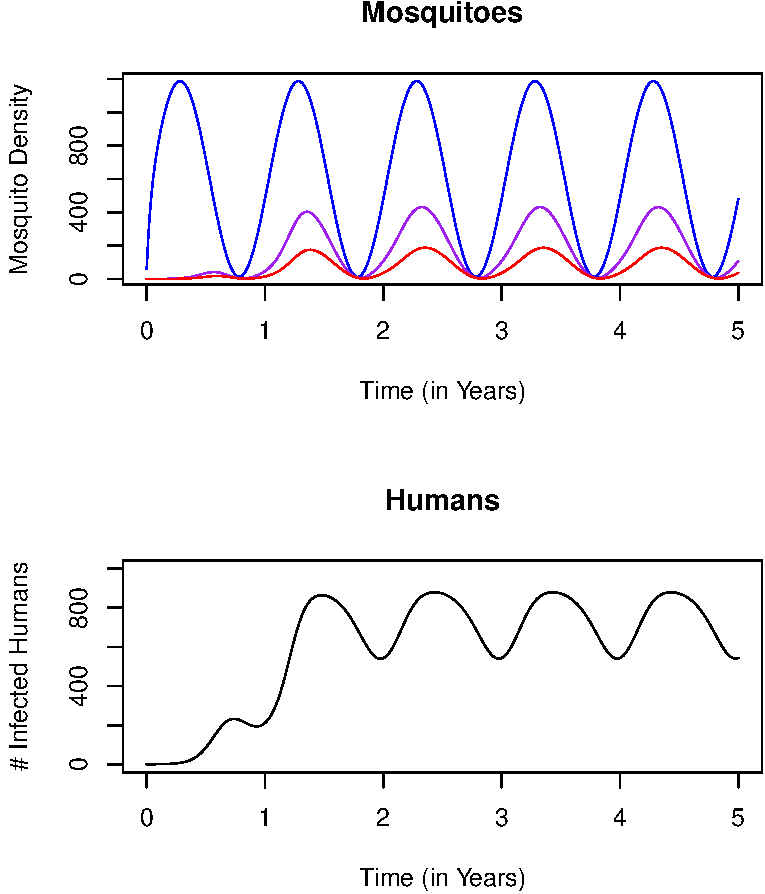
\includegraphics{_main_files/figure-latex/unnamed-chunk-11-1.pdf}
\caption{\label{fig:unnamed-chunk-11}The effect (compare the solid and dashed black lines) and effect size of saturation (blue), graphically.}
\end{figure}

In these formulas, the measure of saturation is exactly \(1+S\kappa\). We could rewrite the relationship between the EIR and VC in a way
that tells us something about how we might be underestimating a parasite's reproductive success:

\[\mbox{EIR}\times (1 + S \kappa) = V \kappa\]
which suggests that each infectious bite is passing along an excess \(S\kappa\) bites.

\hypertarget{malaria-prevalence-thresholds}{%
\subsection{Malaria Prevalence \& Thresholds}\label{malaria-prevalence-thresholds}}

We let \(x\) denote infection prevalence:

\begin{equation}
x = \frac{X}{H} 
\end{equation}

so \(\kappa = c x\), and

\begin{equation}
\frac{dx}{dt} = \frac{1}{H} \frac{dX}{dt} = h (1-x)-r x
\end{equation}

We can also define the basic reproductive number:

\begin{equation}
R_0 = \frac{bcV}{r}.
\end{equation}

It is the product of four terms:

\begin{itemize}
\item
  Vectorial capacity, \(V\), the number of infective bites, per person, per day;
\item
  The number of days a person would remain infectious, \(1/r\);
\item
  The fraction of infectious bites that would infect a human, \(b\);
\item
  The fraction of blood meals on infectious humans that would infect a mosquito, \(c\)
\end{itemize}

After taking their product, we can interpret \(R_0\) as a measure of the parasite's reproductive success after a single generation. It only depends on where we start counting. It could be one of the following:

\begin{itemize}
\item
  the number of infected mosquitoes that would arise from a single infected mosquito;
\item
  the number of infectious mosquitoes that would arise from a single infectious mosquito;
\item
  the number of infected and infectious humans that would arise from a single infected and infectious human.
\end{itemize}

Here, \(R_0\) plays an important role in these equations if we start with \(dX/dt\); then transform it to \(dx/dt\); then replace \(h\) with \(bE\); then replace \(\kappa\) with \(cx\); then divide by \(r\); and rearrange:

\begin{equation}
\frac{1}{r} \frac{dx}{dt} = x \left[R_0 \left(\frac{1-x}{1 + cSx} \right)  - 1\right]  
\end{equation}

Since \(x\) is the prevalence, it is always in the interval \([0,1]\). When \(x\) is very close to \(0\), then

\begin{equation}
\frac{1-x}{1 + cSx} \lesssim 1. 
\end{equation}

and as \(x\) grows very small:

\begin{equation}
\lim_{x \rightarrow 0} \frac{1-x}{1 + cSx} = 1. 
\end{equation}

It follows that when \(x\) is small, \(dx/dt>0\) if and only if \(R_0 > 1\). Depending on \(R_0\), only one of two possibilities can hold:

\begin{itemize}
\item
  either \(R_0<1\), so that \(x=0\) is the steady state;
\item
  or \(R_0 > 1\), and the steady state is:
\end{itemize}

\begin{equation}
\bar x = \frac{R_0 -1}{R_0 + c S} 
\end{equation}

Since at the steady state, \(\kappa = c \bar x\), we can plug this back into the formulas above to get \(\bar Y\) and \(\bar Z\).

What we've learned about these equations is that if mosquito population densities are constant, then malaria reaches a steady state: if \(R_0 >1\), then there is a positive endemic equilibrium, and if \(R_0 < 1\), then malaria is absent from the system. The system is said to be stable -- in fact, is is globally asymptotically stable, which means that all the orbits end up converging to the steady state. This statement has been proved many times in many papers, and since this book is focused on policy, we'll let others worry about proofs.

\hypertarget{checking-our-work}{%
\subsection{Checking our Work}\label{checking-our-work}}

An advantage of working in this environment is that we can check our work. One way we could solve these equations would be to run them for a very long time:

We make a parameter set that defines the model:

\begin{Shaded}
\begin{Highlighting}[]
\NormalTok{y0}\OtherTok{=}\FunctionTok{c}\NormalTok{(}\AttributeTok{M=}\DecValTok{100}\NormalTok{, }\AttributeTok{Y=}\DecValTok{10}\NormalTok{, }\AttributeTok{Z=}\DecValTok{5}\NormalTok{, }\AttributeTok{X=}\DecValTok{200}\NormalTok{)}
\NormalTok{paramsSteady }\OtherTok{=} \FunctionTok{makeParams}\NormalTok{(y0, }\AttributeTok{ss=}\DecValTok{0}\NormalTok{)}
\end{Highlighting}
\end{Shaded}

\begin{Shaded}
\begin{Highlighting}[]
\FunctionTok{dede}\NormalTok{(y0, }\AttributeTok{times=}\NormalTok{tt, }\AttributeTok{func=}\NormalTok{dAronMay, }\AttributeTok{parms=}\NormalTok{paramsSteady) }\OtherTok{{-}\textgreater{}}\NormalTok{ yout}
\FunctionTok{tail}\NormalTok{(yout, }\DecValTok{1}\NormalTok{)[}\SpecialCharTok{{-}}\DecValTok{1}\NormalTok{] }\OtherTok{{-}\textgreater{}}\NormalTok{ eq1 }
\NormalTok{eq1}
\end{Highlighting}
\end{Shaded}

\begin{verbatim}
## [1] 600.00000 211.01706  91.70764 793.10541
\end{verbatim}

By plotting it out, we can check to see if we've run it for long enough:

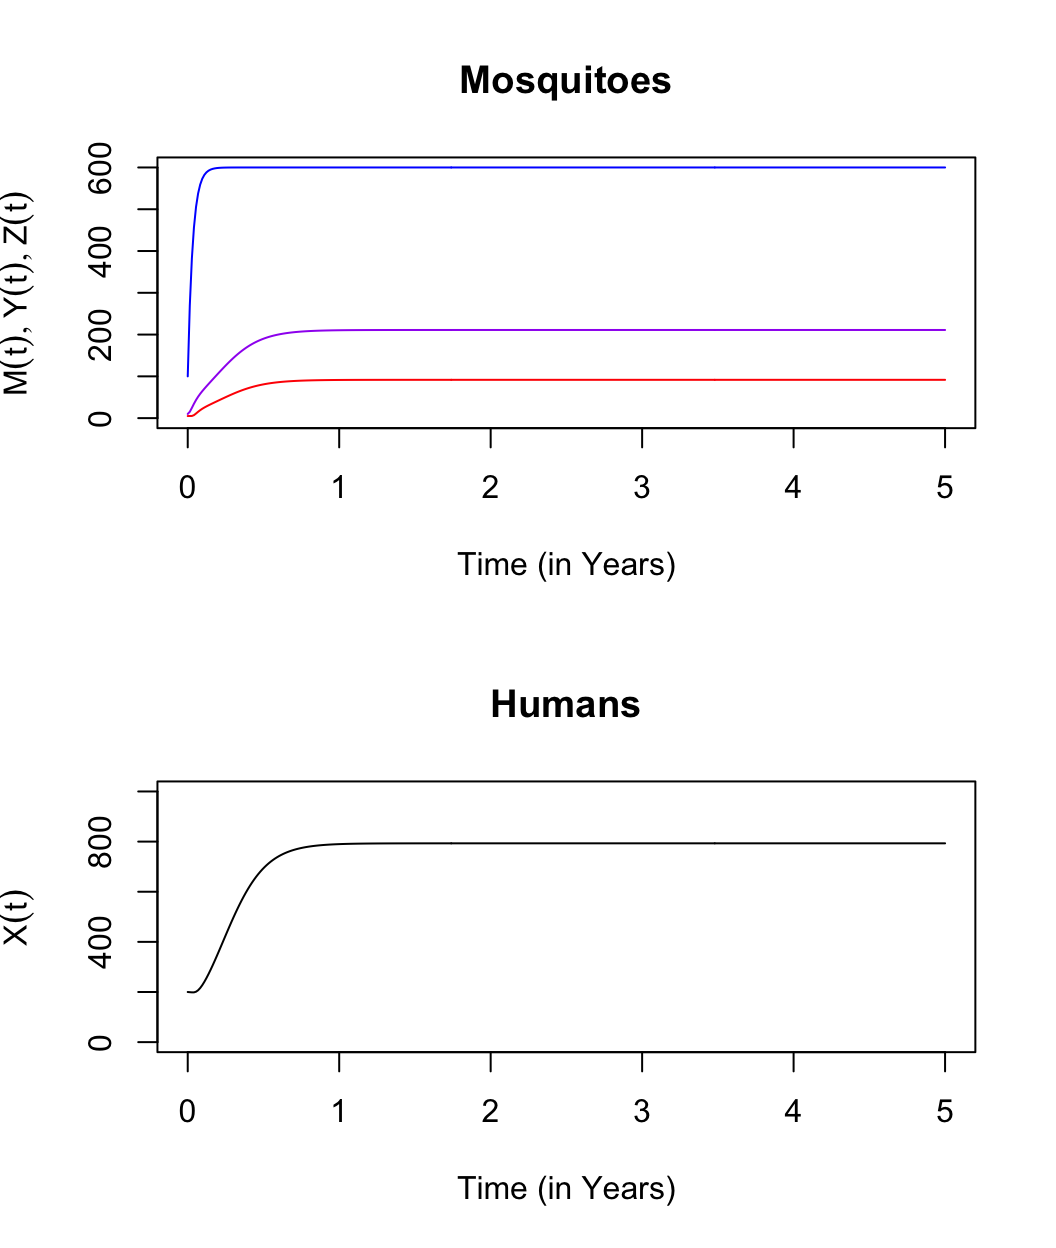
\includegraphics{_main_files/figure-latex/unnamed-chunk-14-1.pdf}

We can check our algebra by computing the same quantities, and \(R_0\) and other quantities we care about:

\begin{Shaded}
\begin{Highlighting}[]
\NormalTok{steadyStates\_AronMay }\OtherTok{=} \ControlFlowTok{function}\NormalTok{(params)\{}\FunctionTok{with}\NormalTok{(params,\{}
\NormalTok{  Lambda }\OtherTok{=}\NormalTok{ m}\SpecialCharTok{*}\NormalTok{H}
\NormalTok{  Meq }\OtherTok{=}\NormalTok{ Lambda}\SpecialCharTok{/}\NormalTok{g}
\NormalTok{  S }\OtherTok{=} \FunctionTok{with}\NormalTok{(paramsSteady, f}\SpecialCharTok{*}\NormalTok{q}\SpecialCharTok{/}\NormalTok{g)}
\NormalTok{  V }\OtherTok{=}\NormalTok{ m}\SpecialCharTok{*}\NormalTok{S}\SpecialCharTok{\^{}}\DecValTok{2}\SpecialCharTok{*}\FunctionTok{exp}\NormalTok{(}\SpecialCharTok{{-}}\NormalTok{g}\SpecialCharTok{*}\NormalTok{tau)}
\NormalTok{  R0 }\OtherTok{=}\NormalTok{ b}\SpecialCharTok{*}\NormalTok{c}\SpecialCharTok{*}\NormalTok{V}\SpecialCharTok{/}\NormalTok{r}
\NormalTok{  x }\OtherTok{=} \FunctionTok{ifelse}\NormalTok{(R0}\SpecialCharTok{\textgreater{}}\DecValTok{1}\NormalTok{,(R0}\DecValTok{{-}1}\NormalTok{)}\SpecialCharTok{/}\NormalTok{(R0}\SpecialCharTok{+}\NormalTok{c}\SpecialCharTok{*}\NormalTok{S), }\DecValTok{0}\NormalTok{) }
\NormalTok{  Xeq }\OtherTok{=}\NormalTok{ x}\SpecialCharTok{*}\NormalTok{H}
\NormalTok{  kappa }\OtherTok{=}\NormalTok{ c}\SpecialCharTok{*}\NormalTok{x}
\NormalTok{  Yeq }\OtherTok{=}\NormalTok{ S}\SpecialCharTok{*}\NormalTok{kappa}\SpecialCharTok{/}\NormalTok{(}\DecValTok{1}\SpecialCharTok{+}\NormalTok{S}\SpecialCharTok{*}\NormalTok{kappa)}\SpecialCharTok{*}\NormalTok{Meq }
\NormalTok{  Zeq }\OtherTok{=}\NormalTok{ Yeq}\SpecialCharTok{*}\FunctionTok{exp}\NormalTok{(}\SpecialCharTok{{-}}\NormalTok{g}\SpecialCharTok{*}\NormalTok{tau) }
\NormalTok{  EIR }\OtherTok{=}\NormalTok{ f}\SpecialCharTok{*}\NormalTok{q}\SpecialCharTok{*}\NormalTok{Zeq}\SpecialCharTok{/}\NormalTok{H}
\NormalTok{  FoI }\OtherTok{=}\NormalTok{ b}\SpecialCharTok{*}\NormalTok{EIR}
\NormalTok{  aEIR }\OtherTok{=} \DecValTok{365}\SpecialCharTok{*}\NormalTok{EIR }
\NormalTok{  aFoI }\OtherTok{=} \DecValTok{365}\SpecialCharTok{*}\NormalTok{FoI }
\NormalTok{  extra}\OtherTok{=}\FunctionTok{c}\NormalTok{(}\AttributeTok{S=}\NormalTok{S, }\AttributeTok{V=}\NormalTok{V, }\AttributeTok{R0=}\NormalTok{R0, }\AttributeTok{x=}\NormalTok{x, }\AttributeTok{kappa=}\NormalTok{kappa, }
          \AttributeTok{EIR=}\NormalTok{EIR, }\AttributeTok{FoI=}\NormalTok{FoI)}
\NormalTok{  annual }\OtherTok{=}\FunctionTok{c}\NormalTok{(}\AttributeTok{aEIR =}\NormalTok{ aEIR, }\AttributeTok{aFoI=}\NormalTok{aFoI)}
  \FunctionTok{list}\NormalTok{(}\AttributeTok{std=}\FunctionTok{c}\NormalTok{(}\AttributeTok{M=}\NormalTok{Meq, }\AttributeTok{Y=}\NormalTok{Yeq, }\AttributeTok{Z=}\NormalTok{Zeq, }\AttributeTok{X=}\NormalTok{Xeq), }
       \AttributeTok{extra=}\FunctionTok{signif}\NormalTok{(extra, }\DecValTok{3}\NormalTok{),}
       \AttributeTok{annual =} \FunctionTok{signif}\NormalTok{(annual,}\DecValTok{3}\NormalTok{)) }
\NormalTok{\})\}}
\FunctionTok{steadyStates\_AronMay}\NormalTok{(paramsSteady) }\OtherTok{{-}\textgreater{}}\NormalTok{ eq2}
\NormalTok{eq2}
\end{Highlighting}
\end{Shaded}

\begin{verbatim}
## $std
##         M         Y         Z         X 
## 600.00000 211.01706  91.70764 793.10541 
## 
## $extra
##      S      V     R0      x  kappa    EIR    FoI 
## 4.5600 0.4520 7.4600 0.7930 0.1190 0.0348 0.0192 
## 
## $annual
## aEIR aFoI 
## 12.7  7.0
\end{verbatim}

Now, we can compare directly:

\begin{Shaded}
\begin{Highlighting}[]
\FunctionTok{rbind}\NormalTok{(}\AttributeTok{eq1=}\NormalTok{eq1, }\AttributeTok{eq2=}\NormalTok{eq2}\SpecialCharTok{$}\NormalTok{std)}
\end{Highlighting}
\end{Shaded}

\begin{verbatim}
##       M        Y        Z        X
## eq1 600 211.0171 91.70764 793.1054
## eq2 600 211.0171 91.70764 793.1054
\end{verbatim}

\hypertarget{stable-orbits}{%
\section{Stable Orbits}\label{stable-orbits}}

If emergence rates vary seasonally, how much of the analysis that we did to understand \emph{steady states} still holds? Obviously, if conditions are changing seasonally, the model does not reach a steady state. In fact, after modification to suit the context, many of the same principles translate. The steady state analysis provides a good qualitative guide, but that the answers will look different. Here, we illustrate by solving systems to illustrate some basic points, which is easy enough. Analysis of the resulting dynamics can be quite difficult; it is covered in {[}Temporal Dynamics{]}.

\hypertarget{thresholds}{%
\subsection{Thresholds}\label{thresholds}}

There is a threshold condition \(R_0>1\) that determines whether malaria is endemic, but the formula for \(R_0\) depends on the form of \(\Lambda(t)\). If we set \(R_0=1\), we can show that the threshold for persistence in a seasonal environment is \(R_0 > \sigma > 1\) (see Figure 1.1). The math to compute threshold conditions in seasonal environments is in {[}Temporal Dynamics{]}.

\begin{figure}
\centering
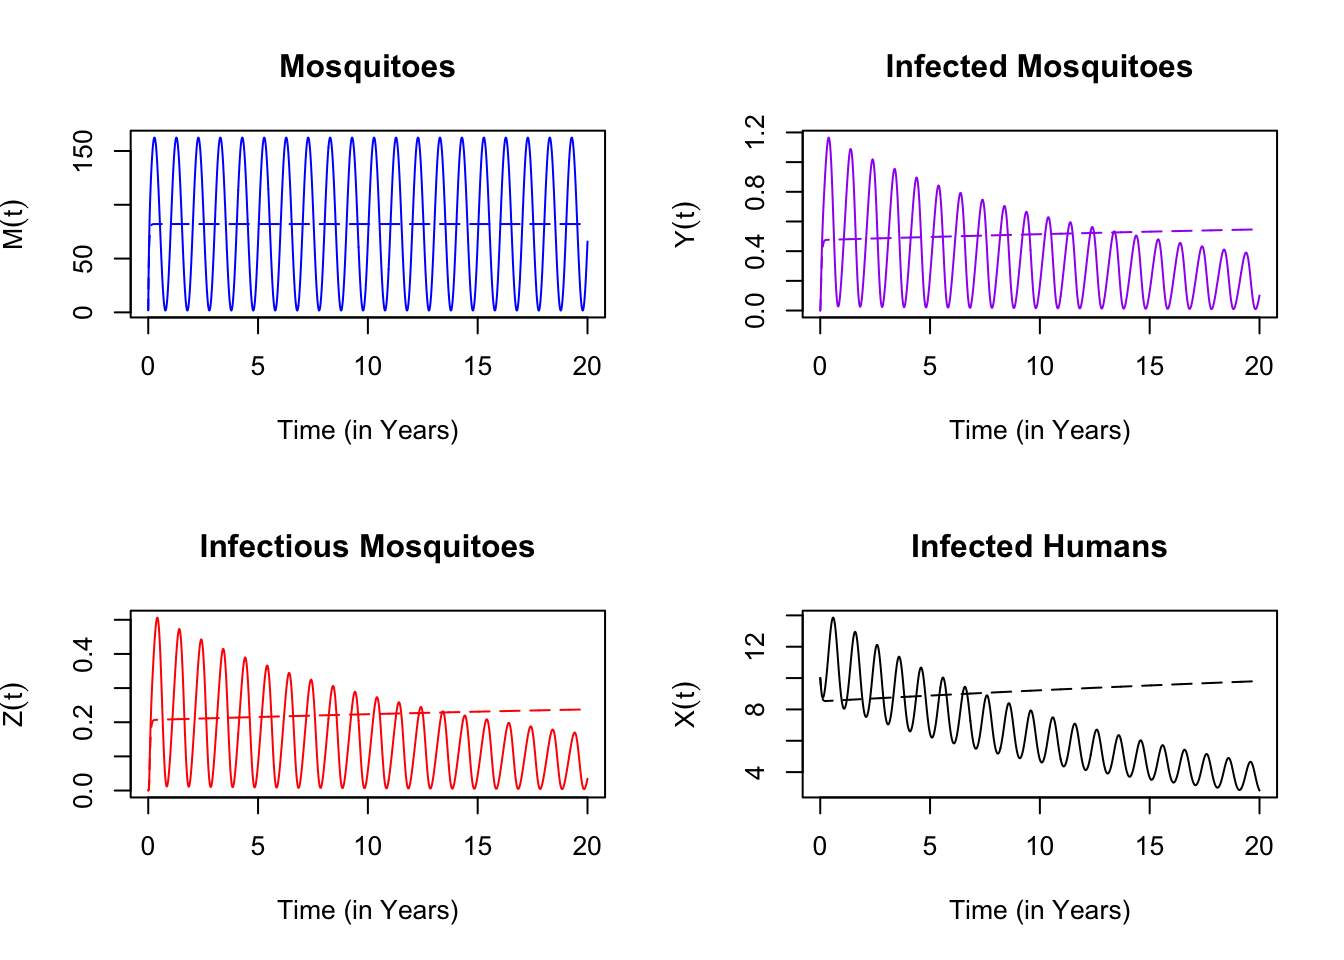
\includegraphics{_main_files/figure-latex/unnamed-chunk-19-1.pdf}
\caption{\label{fig:unnamed-chunk-19}Here, we set \(R_0= 1.02\) for the model with constant emergence, and we show that malaria persists. For the same parameters and for the same \emph{average} emergence rate, malaria declines with seasonality.}
\end{figure}

\clearpage

\hypertarget{orbits}{%
\subsection{Orbits}\label{orbits}}

If \(R_0 >1\), then all orbits converge to a set of \emph{stable orbits} (See Figure 1.1). If \(\Lambda(t)\) has an annual cycle, then after the orbits converge:

\begin{verbatim}
- $M(t+365) = M(t)$; 
- $Y(t+365) = Y(t)$ and $Z(t+365) = Z(t)$; 
- $X(t+365) = X(t)$. 
\end{verbatim}

\begin{figure}
\centering
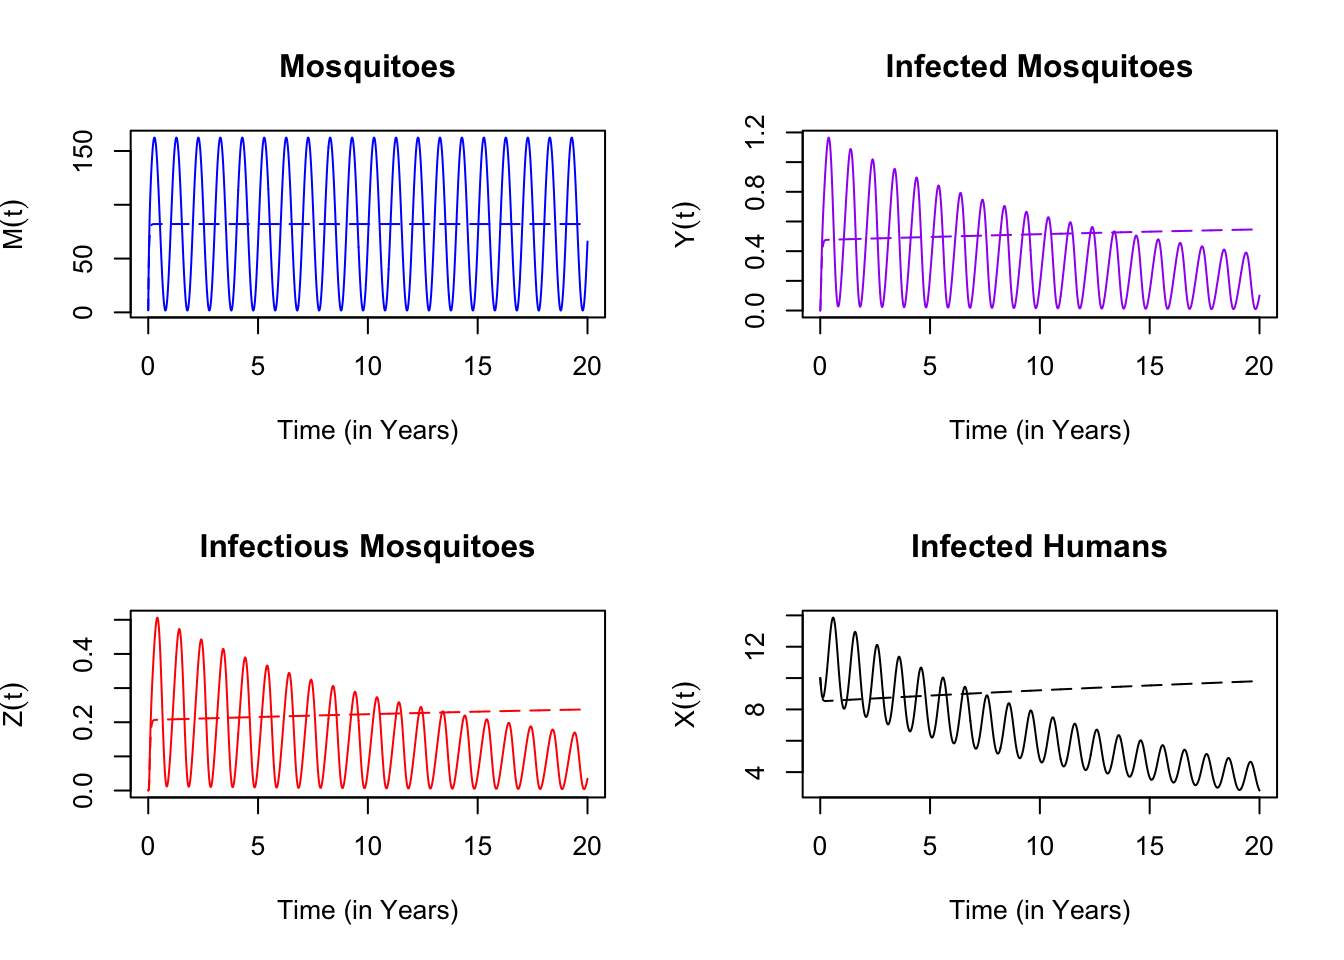
\includegraphics{_main_files/figure-latex/unnamed-chunk-20-1.pdf}
\caption{\label{fig:unnamed-chunk-20}With different initial values, the orbits converge and eventually lie on top of one another.}
\end{figure}

\clearpage

\hypertarget{average-dynamics}{%
\subsection{Average Dynamics}\label{average-dynamics}}

If \(R_0>1\) and malaria is endemic, the \emph{average} prevalence of malaria infection is variable in a seasonal environment. While the prevalence is higher at the peak, the average for the whole year tends to be lower.

\begin{figure}
\centering
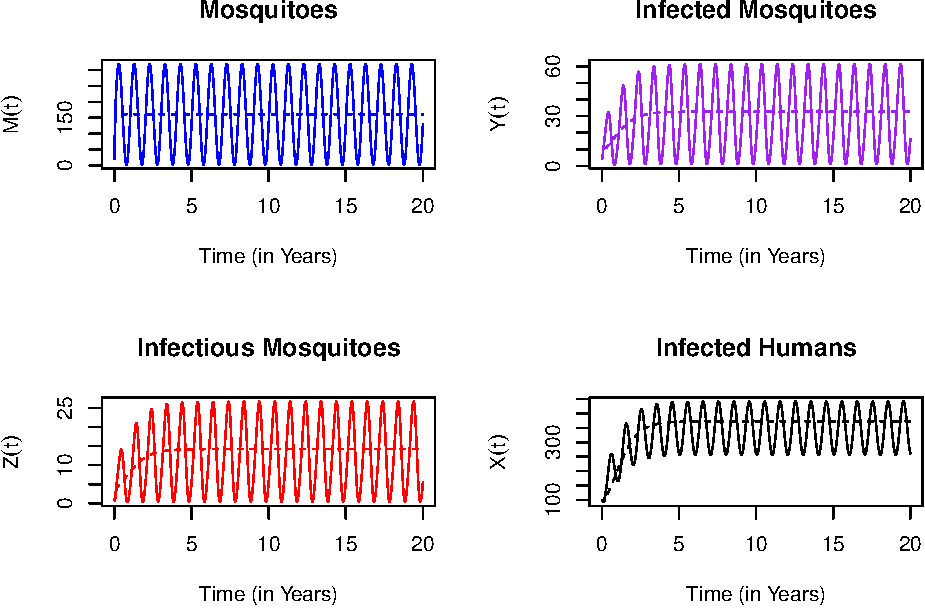
\includegraphics{_main_files/figure-latex/compareTS-1.pdf}
\caption{\label{fig:compareTS}Here, we set \(R_0= 2\) for the model with constant emergence, and we show that the prevalence of malaria is similar in the seasonal environment, but it's higher as transmission peaks, lower in the off-season, and lower overall.}
\end{figure}

\hypertarget{discussion}{%
\section{Discussion}\label{discussion}}

If we were simply learning the math, \ldots{}

When we analyze these equations to determine their \emph{stability} and to identify \emph{threshold conditions,} we focus on threshold conditions and the behavior of these systems when malaria is rare. In most places, malaria is endemic so we need to be concerned about malaria immunity and its effects on transmission; malaria is under some level of control; and because of weather and other factors, the baseline conditions change from year to year.

\hypertarget{mosquito-dynamics}{%
\chapter{Mosquito Dynamics}\label{mosquito-dynamics}}

In the previous chapter, we consider adult mosquito population density as a process closely related to, but also exogenous to the process of parasite transmission. We formulated the models for mosquito density in terms of an emergence rate, \(\Lambda(t)\). In many studies, this might be good enough. There are some challenges in vector control, however, that call for a deeper understanding of adult mosquito population dynamics in relation to the population dynamics of immature mosquito populations. It's hard to imagine giving any advice about LSM without a model of mosquito ecology. Adult vector control will reduce mosquito population densities, but it would also reduce egg laying affecting immature mosquito populations {[}\protect\hyperlink{ref-BradyOJ2015AdultVector}{15}{]}. Mosquito populations have their own thresholds for persistence, and their own spatial dynamics.

While it could be argued that these are not the primary concerns for malaria programs -- we would not disagree -- our mathematical framework must be strong enough to support analytics for integrated vector control, including LSM. Immature mosquito dynamics are one of the core dynamical components in our framework. We introduce the topic here, using a very basic model for mosquito ecology {[}\protect\hyperlink{ref-SmithDL2013_LarvalDynamics}{17}{]}.

To extend the previous model, we need to make several changes and additional assumptions:

\begin{itemize}
\item
  We define terms that describe egg-laying by adult mosquitoes;
\item
  We write a basic equation to describe the dynamics of immature mosquitoes in aquatic habitats as a function of egg-laying. These models describe how eggs hatch, how mosquito larvae develop and mature in aquatic habitats, pupate, and then emerge as adults. The models do not need to be complex, but they could be.
\item
  We replace the parameter \(\Lambda(t)\) from the Aron-May model with a term that
  describes emergence of adults from aquatic habitats.
\end{itemize}

One of the big themes we want to introduce here is that the outcomes of vector control can vary substantially by context because of differences in mosquito ecology.

\hypertarget{aquatic-dynamics}{%
\section{Aquatic Dynamics}\label{aquatic-dynamics}}

\hypertarget{equations}{%
\subsection{Equations}\label{equations}}

Here, we start with the equation for adult ecology from before, leaving out parasite transmission dynamics. We modify the basic slightly by adding one extra term that describes delayed maturation, a different response to crowding {[}\protect\hyperlink{ref-SmithDL2013_LarvalDynamics}{17}{]}. The mosquito maturation rate, \(\psi e^{-\sigma L}\) defines the average time from egg to emergence, and we add one parameter that slows down larval development in response to crowding. The per-capita mortality rate, \(\psi + \theta L\), has two parts: a density independent term \(\psi\) and a response to mean crowding \(\theta L\). We assume that adults lay \(\chi\) eggs per feeding cycle.

\begin{equation}
\begin{array}{rl}
\frac{dM}{dt} &= \Lambda - g M\\  \\ \hline 
\frac{dL}{dt} &= \eta - (\psi e^{-\sigma L} + \phi + \theta L) L \\ 
\Lambda &= \frac{1}{2} \psi L e^{-\sigma L}\\ 
\eta &= \chi f M \\ 
\end{array}
\end{equation}

\hypertarget{solutions-1}{%
\subsection{Solutions}\label{solutions-1}}

\begin{Shaded}
\begin{Highlighting}[]
\NormalTok{BasicAquatic\_dML }\OtherTok{=} \ControlFlowTok{function}\NormalTok{(t, y, params)\{}\FunctionTok{with}\NormalTok{(}\FunctionTok{c}\NormalTok{(params, }\FunctionTok{as.list}\NormalTok{(y)),\{}
   
  \CommentTok{\# Terms }
\NormalTok{  Lambda }\OtherTok{=}\NormalTok{ psi}\SpecialCharTok{*}\FunctionTok{exp}\NormalTok{(}\SpecialCharTok{{-}}\NormalTok{sigma}\SpecialCharTok{*}\NormalTok{L)}\SpecialCharTok{*}\NormalTok{L}\SpecialCharTok{/}\DecValTok{2} 
\NormalTok{  eta }\OtherTok{=}\NormalTok{ chi}\SpecialCharTok{*}\NormalTok{f}\SpecialCharTok{*}\NormalTok{M }
   
  \CommentTok{\# Dynamics }
\NormalTok{  dM }\OtherTok{=}\NormalTok{ Lambda }\SpecialCharTok{{-}}\NormalTok{ g}\SpecialCharTok{*}\NormalTok{M}
\NormalTok{  dL }\OtherTok{=}\NormalTok{ eta }\SpecialCharTok{{-}}\NormalTok{ (psi}\SpecialCharTok{*}\FunctionTok{exp}\NormalTok{(}\SpecialCharTok{{-}}\NormalTok{sigma}\SpecialCharTok{*}\NormalTok{L) }\SpecialCharTok{+}\NormalTok{ phi }\SpecialCharTok{+}\NormalTok{ theta}\SpecialCharTok{*}\NormalTok{L)}\SpecialCharTok{*}\NormalTok{L }
  
  \FunctionTok{return}\NormalTok{(}\FunctionTok{list}\NormalTok{(}\FunctionTok{c}\NormalTok{(dM, dL)))}
\NormalTok{\})\} }
\end{Highlighting}
\end{Shaded}

\begin{Shaded}
\begin{Highlighting}[]
\NormalTok{makePar\_BasicAquatic }\OtherTok{=} \ControlFlowTok{function}\NormalTok{(}\AttributeTok{f=}\DecValTok{1}\SpecialCharTok{/}\FloatTok{2.5}\NormalTok{, }\AttributeTok{g=}\DecValTok{1}\SpecialCharTok{/}\DecValTok{10}\NormalTok{, }\AttributeTok{chi =} \DecValTok{50}\NormalTok{, }\AttributeTok{psi =} \DecValTok{1}\SpecialCharTok{/}\DecValTok{10}\NormalTok{, }\AttributeTok{phi =} \DecValTok{1}\SpecialCharTok{/}\DecValTok{10}\NormalTok{, }\AttributeTok{theta =} \DecValTok{1}\SpecialCharTok{/}\DecValTok{100}\NormalTok{, }\AttributeTok{sigma=}\DecValTok{0}\NormalTok{)\{}
  \FunctionTok{list}\NormalTok{(}\AttributeTok{f=}\NormalTok{f, }\AttributeTok{g=}\NormalTok{g, }\AttributeTok{chi=}\NormalTok{chi, }\AttributeTok{psi=}\NormalTok{psi, }\AttributeTok{phi=}\NormalTok{phi, }\AttributeTok{theta=}\NormalTok{theta, }\AttributeTok{sigma=}\NormalTok{sigma)}
\NormalTok{\}}
\end{Highlighting}
\end{Shaded}

\hypertarget{regulation}{%
\subsection{Regulation}\label{regulation}}

\begin{Shaded}
\begin{Highlighting}[]
\NormalTok{tt }\OtherTok{=} \FunctionTok{seq}\NormalTok{(}\DecValTok{0}\NormalTok{,}\DecValTok{100}\NormalTok{, }\AttributeTok{by=}\DecValTok{1}\NormalTok{) }
\NormalTok{y0 }\OtherTok{=} \FunctionTok{c}\NormalTok{(}\AttributeTok{M=}\DecValTok{1}\NormalTok{, }\AttributeTok{L=}\DecValTok{1}\NormalTok{)}
\NormalTok{params }\OtherTok{=} \FunctionTok{makePar\_BasicAquatic}\NormalTok{()}
\NormalTok{params1 }\OtherTok{=} \FunctionTok{makePar\_BasicAquatic}\NormalTok{(}\AttributeTok{phi=}\DecValTok{1}\NormalTok{)}
\NormalTok{params2 }\OtherTok{=} \FunctionTok{makePar\_BasicAquatic}\NormalTok{(}\AttributeTok{theta=}\DecValTok{1}\SpecialCharTok{/}\DecValTok{10}\NormalTok{)}
\NormalTok{params3 }\OtherTok{=} \FunctionTok{makePar\_BasicAquatic}\NormalTok{(}\AttributeTok{sigma=}\DecValTok{1}\SpecialCharTok{/}\DecValTok{100}\NormalTok{, }\AttributeTok{theta=}\DecValTok{0}\NormalTok{)}
\end{Highlighting}
\end{Shaded}

This code solves the equations:

\begin{Shaded}
\begin{Highlighting}[]
\FunctionTok{require}\NormalTok{(deSolve)}
\NormalTok{yout  }\OtherTok{\textless{}{-}} \FunctionTok{lsode}\NormalTok{(}\AttributeTok{y=}\NormalTok{y0, }\AttributeTok{times=}\NormalTok{tt, }\AttributeTok{func=}\NormalTok{BasicAquatic\_dML, }\AttributeTok{parms=}\NormalTok{params) }
\NormalTok{yout1 }\OtherTok{\textless{}{-}} \FunctionTok{lsode}\NormalTok{(}\AttributeTok{y=}\NormalTok{y0, }\AttributeTok{times=}\NormalTok{tt, }\AttributeTok{func=}\NormalTok{BasicAquatic\_dML, }\AttributeTok{parms=}\NormalTok{params1) }
\NormalTok{yout2 }\OtherTok{\textless{}{-}} \FunctionTok{lsode}\NormalTok{(}\AttributeTok{y=}\NormalTok{y0, }\AttributeTok{times=}\NormalTok{tt, }\AttributeTok{func=}\NormalTok{BasicAquatic\_dML, }\AttributeTok{parms=}\NormalTok{params2) }
\NormalTok{yout3 }\OtherTok{\textless{}{-}} \FunctionTok{lsode}\NormalTok{(}\AttributeTok{y=}\NormalTok{y0, }\AttributeTok{times=}\NormalTok{tt, }\AttributeTok{func=}\NormalTok{BasicAquatic\_dML, }\AttributeTok{parms=}\NormalTok{params3) }
\end{Highlighting}
\end{Shaded}

\begin{Shaded}
\begin{Highlighting}[]
\NormalTok{plotML }\OtherTok{=} \ControlFlowTok{function}\NormalTok{(out, }\AttributeTok{llwd=}\DecValTok{1}\NormalTok{, }\AttributeTok{clrL =} \StringTok{"blue"}\NormalTok{, }\AttributeTok{clrM=}\StringTok{"red"}\NormalTok{)\{}\FunctionTok{with}\NormalTok{(}\FunctionTok{data.frame}\NormalTok{(out),\{}
  \FunctionTok{plot}\NormalTok{(time, L, }\AttributeTok{type =} \StringTok{"l"}\NormalTok{, }\AttributeTok{lwd=}\NormalTok{llwd, }\AttributeTok{col =}\NormalTok{ clrL, }\AttributeTok{xlab =} \StringTok{"Time (Days)"}\NormalTok{, }\AttributeTok{ylab =} \StringTok{"Density"}\NormalTok{) }
  \FunctionTok{lines}\NormalTok{(time, M, }\AttributeTok{col =}\NormalTok{ clrM, }\AttributeTok{lwd=}\NormalTok{llwd) }
\NormalTok{\})\}}

\NormalTok{addML }\OtherTok{=} \ControlFlowTok{function}\NormalTok{(out, }\AttributeTok{llty =} \DecValTok{2}\NormalTok{, }\AttributeTok{llwd=}\DecValTok{1}\NormalTok{, }\AttributeTok{clrL =} \StringTok{"blue"}\NormalTok{, }\AttributeTok{clrM=}\StringTok{"red"}\NormalTok{)\{}\FunctionTok{with}\NormalTok{(}\FunctionTok{data.frame}\NormalTok{(out),\{}
  \FunctionTok{lines}\NormalTok{(time, L, }\AttributeTok{col =}\NormalTok{ clrL, }\AttributeTok{lty=}\NormalTok{llty, }\AttributeTok{lwd=}\NormalTok{llwd) }
  \FunctionTok{lines}\NormalTok{(time, M, }\AttributeTok{col =}\NormalTok{ clrM, }\AttributeTok{lty=}\NormalTok{llty, }\AttributeTok{lwd=}\NormalTok{llwd) }
\NormalTok{\})\}}
\end{Highlighting}
\end{Shaded}

The first thing to point out is that changing the dynamics take some time to approach equilibrium -- a couple of months, in this model. The second is that increasing mortality rates for mosquitoes in aquatic habitats by a factor of 10 affects the mosquito densities in minor ways.

\begin{Shaded}
\begin{Highlighting}[]
\FunctionTok{plotML}\NormalTok{(yout)}
\FunctionTok{addML}\NormalTok{(yout1, }\AttributeTok{clrL =} \StringTok{"darkblue"}\NormalTok{, }\AttributeTok{clrM=}\StringTok{"darkred"}\NormalTok{, }\AttributeTok{llwd=}\FloatTok{1.5}\NormalTok{)}
\end{Highlighting}
\end{Shaded}

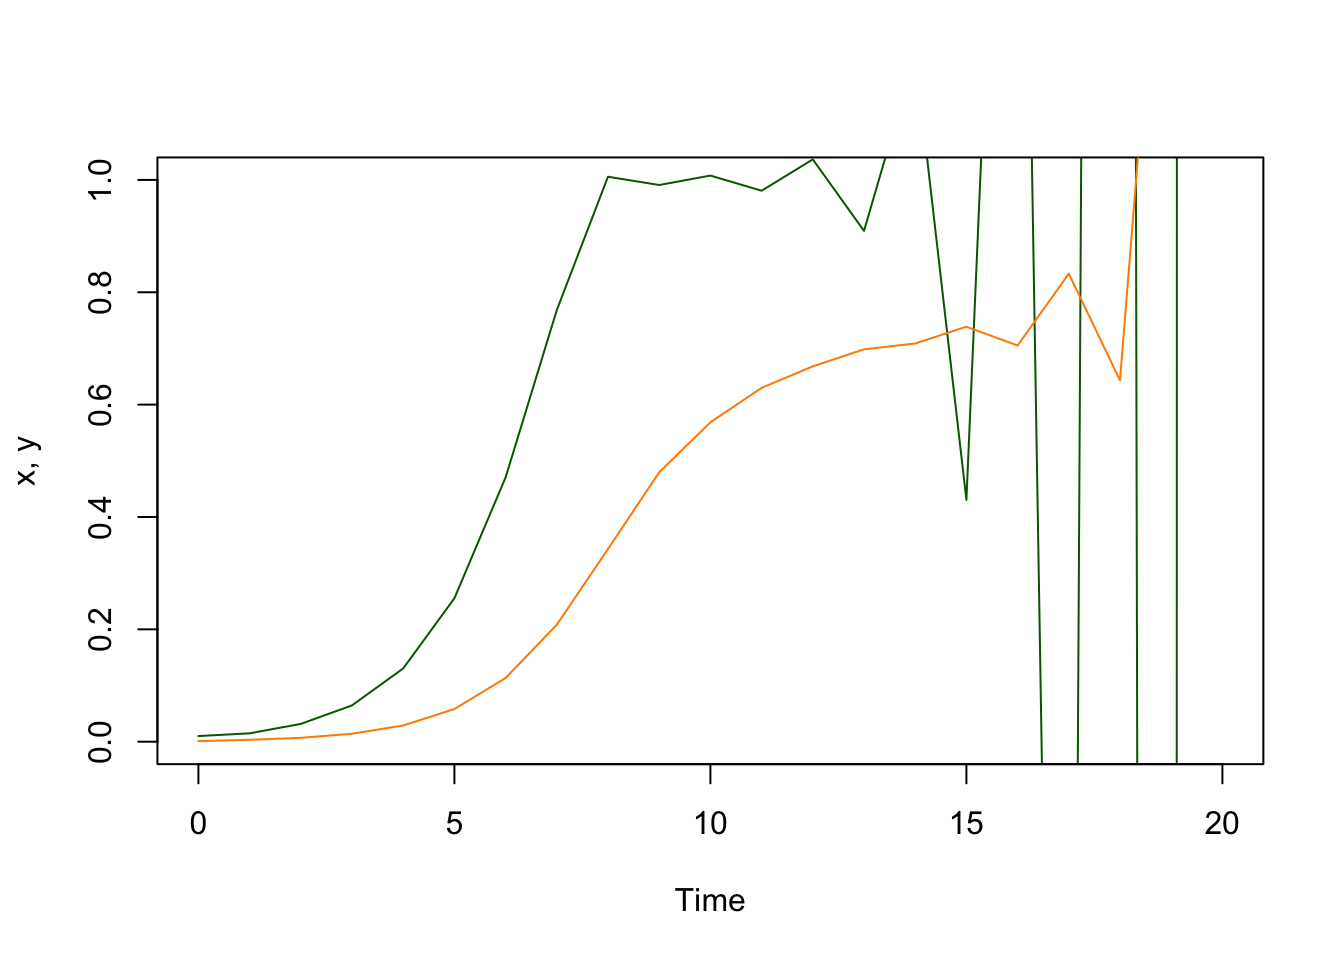
\includegraphics{_main_files/figure-latex/unnamed-chunk-25-1.pdf}

The third is that increasing the response to mean crowding has a very strong effect on the population dynamics.

\begin{Shaded}
\begin{Highlighting}[]
\FunctionTok{plotML}\NormalTok{(yout)}
\FunctionTok{addML}\NormalTok{(yout2, }\AttributeTok{clrL =} \StringTok{"darkblue"}\NormalTok{, }\AttributeTok{clrM=}\StringTok{"darkred"}\NormalTok{, }\AttributeTok{llwd=}\FloatTok{1.5}\NormalTok{)}
\end{Highlighting}
\end{Shaded}

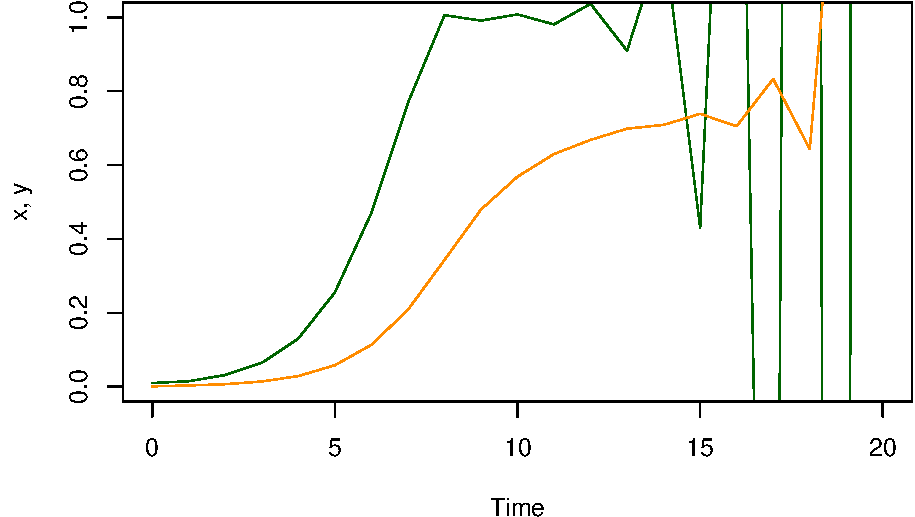
\includegraphics{_main_files/figure-latex/unnamed-chunk-26-1.pdf}

The third point is that density dependent responses to mean crowding cause much larger changes to this system than density-dependent mortality. Aquatic dynamics have a strong tendency to oscillate, but more critically, delayed maturation strongly affects the ratio of adult mosquitoes to adults.

\begin{Shaded}
\begin{Highlighting}[]
\FunctionTok{plotML}\NormalTok{(yout)}
\FunctionTok{addML}\NormalTok{(yout3, }\AttributeTok{clrL =} \StringTok{"darkblue"}\NormalTok{, }\AttributeTok{clrM=}\StringTok{"darkred"}\NormalTok{, }\AttributeTok{llwd=}\FloatTok{1.5}\NormalTok{)}
\end{Highlighting}
\end{Shaded}

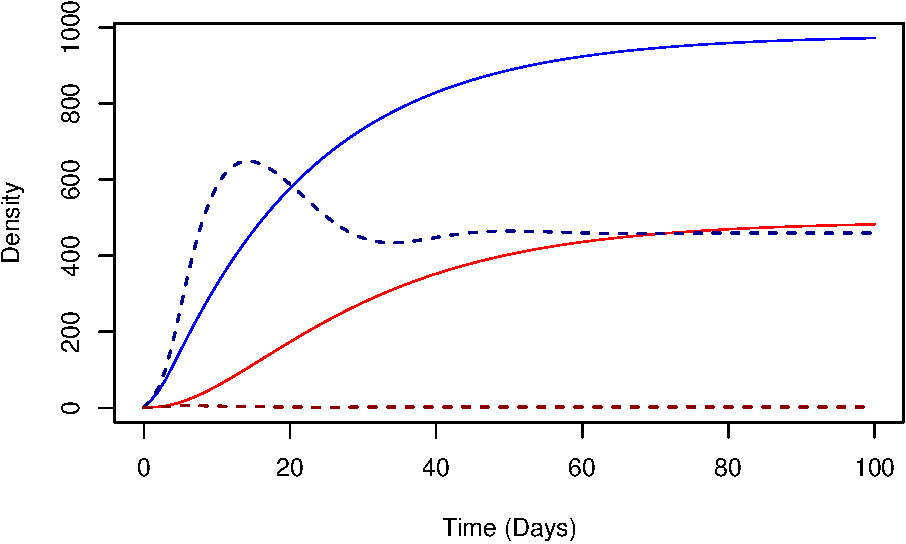
\includegraphics{_main_files/figure-latex/compareML-1.pdf}

\begin{Shaded}
\begin{Highlighting}[]
\FunctionTok{plot}\NormalTok{(}\DecValTok{1}\NormalTok{,}\DecValTok{1}\NormalTok{)}
\end{Highlighting}
\end{Shaded}

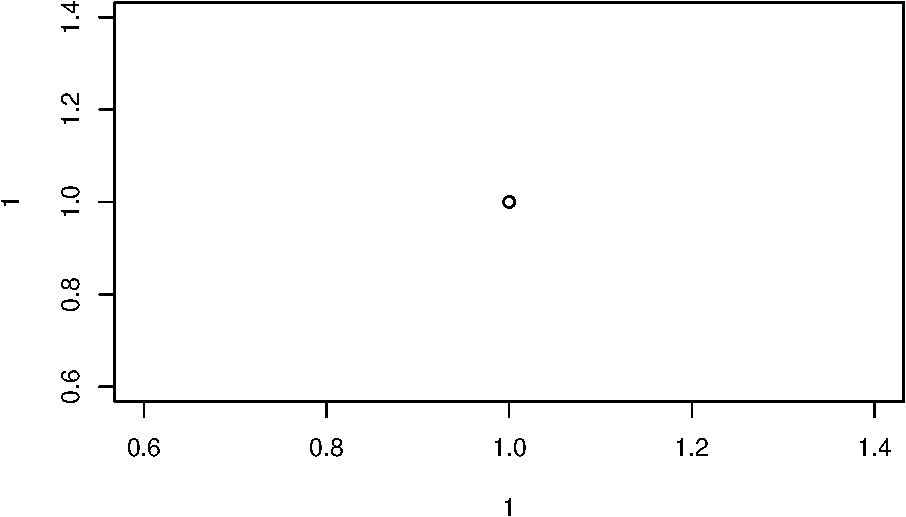
\includegraphics{_main_files/figure-latex/test-1.pdf}

\hypertarget{understanding-mosquito-dynamics}{%
\section{Understanding Mosquito Dynamics}\label{understanding-mosquito-dynamics}}

This

\hypertarget{part-supplements}{%
\part{Supplements}\label{part-supplements}}

\hypertarget{references}{%
\chapter{References}\label{references}}

If you want a PDF and can't find it at the link provided, let us know and we can help you find a copy.

\hypertarget{refs}{}
\begin{CSLReferences}{0}{0}
\leavevmode\vadjust pre{\hypertarget{ref-SmithDL2012_RossMacdonald}{}}%
\CSLLeftMargin{1. }%
\CSLRightInline{Smith DL, Battle KE, Hay SI, Barker CM, Scott TW, McKenzie FE. Ross, {Macdonald}, and a theory for the dynamics and control of mosquito-transmitted pathogens. PLoS Pathog. 2012;8: e1002588. doi:\href{https://doi.org/10.1371/journal.ppat.1002588}{10.1371/journal.ppat.1002588}}

\leavevmode\vadjust pre{\hypertarget{ref-SmithNR2018AgentbasedModels}{}}%
\CSLLeftMargin{2. }%
\CSLRightInline{Smith NR, Trauer JM, Gambhir M, Richards JS, Maude RJ, Keith JM, et al. Agent-based models of malaria transmission: {A} systematic review. Malar J. 2018;17: 299. doi:\href{https://doi.org/10.1186/s12936-018-2442-y}{10.1186/s12936-018-2442-y}}

\leavevmode\vadjust pre{\hypertarget{ref-SmithDL2014_Recasting}{}}%
\CSLLeftMargin{3. }%
\CSLRightInline{Smith DL, Perkins TA, Reiner RC Jr, Barker CM, Niu T, Chaves LF, et al. Recasting the theory of mosquito-borne pathogen transmission dynamics and control. Trans R Soc Trop Med Hyg. 2014;108: 185--197. doi:\href{https://doi.org/10.1093/trstmh/tru026}{10.1093/trstmh/tru026}}

\leavevmode\vadjust pre{\hypertarget{ref-CarterR2002SpatialSimulation}{}}%
\CSLLeftMargin{4. }%
\CSLRightInline{Carter R. Spatial simulation of malaria transmission and its control by malaria transmission blocking vaccination. International Journal for Parasitology. 2002;32: 1617--1624. doi:\href{https://doi.org/10.1016/S0020-7519(02)00190-X}{10.1016/S0020-7519(02)00190-X}}

\leavevmode\vadjust pre{\hypertarget{ref-GuW2003IndividualbasedModel}{}}%
\CSLLeftMargin{5. }%
\CSLRightInline{Gu W, Killeen GF, Mbogo CM, Regens JL, Githure JI, Beier JC. An individual-based model of \emph{{Plasmodium} falciparum} malaria transmission on the coast of {Kenya}. Trans R Soc Trop Med Hyg. 2003;97: 43--50. doi:\href{https://doi.org/10.1016/s0035-9203(03)90018-6}{10.1016/s0035-9203(03)90018-6}}

\leavevmode\vadjust pre{\hypertarget{ref-PerkinsTA2013HeterogeneityMixing}{}}%
\CSLLeftMargin{6. }%
\CSLRightInline{Perkins TA, Scott TW, Le Menach A, Smith DL. Heterogeneity, mixing, and the spatial scales of mosquito-borne pathogen transmission. PLoS Comput Biol. 2013;9: e1003327. }

\leavevmode\vadjust pre{\hypertarget{ref-TatemAJ2010InternationalPopulation}{}}%
\CSLLeftMargin{7. }%
\CSLRightInline{Tatem AJ, Smith DL. International population movements and regional \emph{{Plasmodium} falciparum} malaria elimination strategies. Proc Natl Acad Sci U S A. 2010;107: 12222--12227. doi:\href{https://doi.org/10.1073/pnas.1002971107}{10.1073/pnas.1002971107}}

\leavevmode\vadjust pre{\hypertarget{ref-WuSL2020MBITES}{}}%
\CSLLeftMargin{8. }%
\CSLRightInline{Wu SL, Sánchez C HM, Henry JM, Citron DT, Zhang Q, Compton K, et al. Vector bionomics and vectorial capacity as emergent properties of mosquito behaviors and ecology. PLoS Comput Biol. 2020;16: e1007446. doi:\href{https://doi.org/10.1371/journal.pcbi.1007446}{10.1371/journal.pcbi.1007446}}

\leavevmode\vadjust pre{\hypertarget{ref-WuSL2022SpatialDynamics}{}}%
\CSLLeftMargin{9. }%
\CSLRightInline{Wu SL, Henry JM, Citron DT, Mbabazi Ssebuliba D, Nakakawa Nsumba J, Sánchez C. HM, et al. Spatial {Dynamics} of {Malaria} {Transmission}. 2022. Available: \url{http://medrxiv.org/content/early/2022/11/15/2022.11.07.22282044.abstract}}

\leavevmode\vadjust pre{\hypertarget{ref-RossR1905LogicalBasis}{}}%
\CSLLeftMargin{10. }%
\CSLRightInline{Ross R. The logical basis of the sanitary policy of mosquito reduction. Science. 1905;22: 689--699. doi:\href{https://doi.org/10.1126/science.22.570.689}{10.1126/science.22.570.689}}

\leavevmode\vadjust pre{\hypertarget{ref-RossR1908ReportPrevention}{}}%
\CSLLeftMargin{11. }%
\CSLRightInline{Ross R. Report on the {Prevention} of {Malaria} in {Mauritius}. London: Waterlow; 1908. Available: \url{https://play.google.com/store/books/details?id=0Mc1AQAAMAAJ}}

\leavevmode\vadjust pre{\hypertarget{ref-AronJL1982PopulationDynamics}{}}%
\CSLLeftMargin{12. }%
\CSLRightInline{Aron JL, May RM. The population dynamics of malaria. In: Anderson RM, editor. The {Population} {Dynamics} of {Infectious} {Diseases}: {Theory} and {Applications}. Boston, MA: Springer US; 1982. pp. 139--179. doi:\href{https://doi.org/10.1007/978-1-4899-2901-3_5}{10.1007/978-1-4899-2901-3\_5}}

\leavevmode\vadjust pre{\hypertarget{ref-SmithDL2004_Statics}{}}%
\CSLLeftMargin{13. }%
\CSLRightInline{Smith DL, McKenzie FE. Statics and dynamics of malaria infection in {Anopheles} mosquitoes. Malaria Journal. 2004;3: 13. doi:\href{https://doi.org/10.1186/1475-2875-3-13}{10.1186/1475-2875-3-13}}

\leavevmode\vadjust pre{\hypertarget{ref-SmithDL2021_NewTestOldMosquitoes}{}}%
\CSLLeftMargin{14. }%
\CSLRightInline{Smith DL, Musiime AK, Maxwell K, Lindsay SW, Kiware S. A {New} {Test} of a {Theory} about {Old} {Mosquitoes}. Trends Parasitol. 2021;37: 185--194. doi:\href{https://doi.org/10.1016/j.pt.2020.10.011}{10.1016/j.pt.2020.10.011}}

\leavevmode\vadjust pre{\hypertarget{ref-BradyOJ2015AdultVector}{}}%
\CSLLeftMargin{15. }%
\CSLRightInline{Brady OJ, Godfray HCJ, Tatem AJ, Gething PW, Cohen JM, McKenzie FE, et al. Adult vector control, mosquito ecology and malaria transmission. International Health. 2015;7: 121--129. doi:\href{https://doi.org/10.1093/inthealth/ihv010}{10.1093/inthealth/ihv010}}

\leavevmode\vadjust pre{\hypertarget{ref-MacdonaldG1952_SporozoiteRate}{}}%
\CSLLeftMargin{16. }%
\CSLRightInline{Macdonald G. The analysis of the sporozoite rate. Trop Dis Bull. 1952;49: 569--586. Available: \url{https://www.ncbi.nlm.nih.gov/pubmed/14958825}}

\leavevmode\vadjust pre{\hypertarget{ref-SmithDL2013_LarvalDynamics}{}}%
\CSLLeftMargin{17. }%
\CSLRightInline{Smith DL, Perkins TA, Tusting LS, Scott TW, Lindsay SW. Mosquito {Population} {Regulation} and {Larval} {Source} {Management} in {Heterogeneous} {Environments}. PLOS ONE. 2013;8: e71247. doi:\href{https://doi.org/10.1371/journal.pone.0071247}{10.1371/journal.pone.0071247}}

\end{CSLReferences}

\end{document}
